\documentclass[12pt, a4paper]{article}

% Text languages
\usepackage[english, UKenglish, USenglish, american, british]{babel}

% Accents
%usepackage[latin1]{inputenc}

% Maths
\usepackage{mathtools}
\usepackage{amsmath,amsthm,amssymb}

% Double rows
%\usepackage{multirow}

% Math-mode symbol & verbatim
%\def\W#1#2{$#1{#2}$ &\tt\string#1\string{#2\string}}
%\def\X#1{$#1$ &\tt\string#1}
%\def\Y#1{$\big#1$ &\tt\string#1}
%\def\Z#1{\tt\string#1}

% A non-floating table environment.
%\makeatletter
%\renewenvironment{table}%
%   {\vskip\intextsep\parskip\z@
%    \vbox\bgroup\centering\def\@captype{table}}%
%   {\egroup\vskip\intextsep}
%\makeatother

%\DeclarePairedDelimiter\abs{\lvert}{\rvert}%
%\DeclarePairedDelimiter\norm{\lVert}{\rVert}%

% Swap the definition of \abs* and \norm*, so that \abs
% and \norm resizes the size of the brackets, and the 
% starred version does not.
%\makeatletter
%\let\oldabs\abs
%\def\abs{\@ifstar{\oldabs}{\oldabs*}}
%
%\let\oldnorm\norm
%\def\norm{\@ifstar{\oldnorm}{\oldnorm*}}
%\makeatother

% C++
\usepackage{listings}
\usepackage{xcolor}
\lstset { %
	language = C++,
	backgroundcolor=\color{black!5}, % set backgroundcolor
    basicstyle=\footnotesize,% basic font setting
    tabsize=4, % tab space width
    showstringspaces=false, % don't mark spaces in strings
    %numbers=left, % display line numbers on the left
    commentstyle=\color{green}, % comment color
    keywordstyle=\color{blue}, % keyword color
    stringstyle=\color{red} % string color
}

% https://www.overleaf.com/learn/latex/Page_size_and_margins
\usepackage{geometry}
\topmargin = -23pt
\oddsidemargin = 13pt
\headheight = 12pt
\headsep = 25pt
\textheight = 674pt
\textwidth = 426pt
\marginparsep = 10pt
\marginparwidth = 50pt
\footskip = 30pt
\marginparpush = 5pt
\hoffset = 0pt
\voffset = 0pt
\paperwidth = 597pt
\paperheight = 845pt

% Hyperlinks
\usepackage{hyperref}

% Figure
\usepackage{graphicx}
\usepackage{caption}
\usepackage{subcaption}
\usepackage{etoc}
% Example
\newtheorem{exmp}{Example}[section]
% Algorithms
%\usepackage[]{algorithm2e}
%\usepackage{algorithm}% http://ctan.org/pkg/algorithm
%\usepackage{algpseudocode}% http://ctan.org/pkg/algorithmicx
\usepackage{algpseudocode}

\renewcommand{\thefootnote}{\arabic{footnote}} % 1, 2, 3... (la que hay por defecto)

\setcounter{secnumdepth}{5}
\setcounter{tocdepth}{5}

%\titleformat{\paragraph}
%{\normalfont\normalsize\bfseries}{\theparagraph}{1em}{}
%\titlespacing*{\paragraph}
%{0pt}{3.25ex plus 1ex minus .2ex}{1.5ex plus .2ex}

\usepackage{float}
%--------------------------------------------------------------------------
\title{PARALLELISM}
\author{Roger Vilaseca Darné and Xavier Martín Ballesteros\\
  \small UNIVERSITAT POLITÈCNICA DE CATALUNYA\\
}
\date{10th December 2018}

\begin{document}
% Images
\graphicspath{ {./images} }

%\maketitle

\begin{titlepage}
	\centering
%	{\scshape\LARGE UNIVERSITAT POLITÈCNICA DE CATALUNYA \par}
	\vspace{1cm}
	{\scshape\Large UNIVERSITAT POLITECNICA DE CATALUNYA\par}
	\vspace{1.5cm}
	{\huge\bfseries PARALLELISM\par}
	\vspace{2cm}
	{\Large\itshape \textbf{Lab 3: Embarrassingly parallelism with OpenMP: Mandelbrot set}\par}
	\vfill
	{\Large\itshape Roger Vilaseca Darne and Xavier Martin Ballesteros\break PAR4110\par}
	\vfill
	
\includegraphics[width=0.25\textwidth]{./images/UPC.png}\par\vspace{1cm}
	%supervised by\par
	%Dr.~Mark \textsc{Brown}

	\vfill

% Bottom of the page
	{\large 10th April 2019, Q2}
\end{titlepage}

%\abstract{Esto es una plantilla simple para un articulo en \LaTeX.}

%	*********************** ÍNDEX *********************
\setcounter{secnumdepth}{5}

\newpage
  \tableofcontents
\newpage

% Referència a una equació \ref{eq:area}).
% Referència a una secció \ref{sec:nada}
% Referència a una cita \cite{Cd94}.

\section{Introduction}

Nowadays, the aim of parallelizing codes is to improve the performance of nearly all the applications that can be computed using classical computer architectures. Nevertheless, there are several ways to parallelize the same application, some better than others.

In our case, we are going to study different tasking models in OpenMP to parallelize the Mandelbrot set, a particular set of point, in the complex domain, whose boundary generates a distinctive and easily recognisable two-dimensional fractal shape\footnote{To know more about the Mnadelbrot set, it is highly recommended to look at the following link: \url{http://en.wikipedia.org/wiki/Mandelbrot\_set}}.

Based on the maximum number of steps the code does to calculate wheater a point belongs to the set or not, the coloring of the image changes. The points that belong to the set reach the maximum limit of steps. In the figure \ref{mandelbrot}, those points are the ones in black color. Hence, the points which are not black are the ones that do not belong to the set.

\begin{figure}[H]
	\centering
	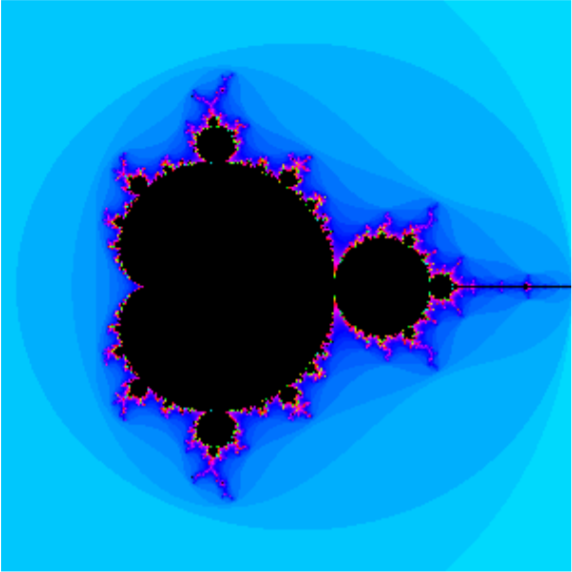
\includegraphics[scale=0.7]{./mandelbrotset}
	\caption{Fractal shape.}
	\label{mandelbrot}
\end{figure}

First of all we are going to see with \textit{Tareador} the binaries which are potentailly parallelizable. Afterwards, we are going to explore two parallelization methods: Point and Row decomposition. To do it, we are going to use the following tasking models: explicit task implementation (task only, task with taskwait/taskgroup/taskloop) and implicit task implementation (for-based implementation). Finally, we are going to compare the best implementation of one method with the best implementation of the other one.

\newpage

\section{Task decomposition analysis with \textit{Tareador}}
\label{sec:tareador}

In this section, we had to analyse the two possible task granularities that could be exploited in the given program. To do it, we used the \textit{Tareador} tool, which was very useful to see graphically the created tasks and which dependences exist between them.

\subsection{Point decomposition}

In this decomposition strategy, a task corresponds with the computation of a single point (row, col) of the Mandelbrot set. Thus, we will have $row \times col$ tasks.

In order to analyse the potential parallelism of this strategy, we modified the code in \textit{mandel-tar.c} to create several \textit{Tareador} tasks. As we are using a point decomposition strategy, the tasks are created inside the most inner loop of the function mandelbrot.  Figure \ref{code:mandeltarPoint} shows the fragment of the function that we modified.

\begin{figure}[H]
\begin{lstlisting}
for (row = 0; row < height; ++row) {
	for (col = 0; col < width; ++col) {
		tareador_start_task("point");
		
		...
		
		tareador_end_task("point");
	}
}
\end{lstlisting}
\caption{Modified fragment of the \textit{mandel-tar.c} code.}
\label{code:mandeltarPoint}
\end{figure}

Once we did this, we executed interactively mandeld-tar and mandel-tar using run-tareador.sh script. The first one is used for timing purposes and to check for the numerical validity of the output (-o option) whereas with the second one we can visualize the Mandelbrot set.

The script has defined inside the size of the image to compute (-w option). In this case, the value was 8 to generate a reasonable task graph in a reasonable execution time. Hence, as we said before, the number of tasks will be $8 \times 8 = 64$.

Figures \ref{fig:mandel-tar-point} and \ref{fig:mandeld-tar-point} below show the two task decomposition graphs (TDG) of the two possible executions. There are some nodes bigger than the others. This is because these nodes have executed more instructions than the rest. Therefore, these nodes represent pixels in white\footnote{The bigger the node, the more iterations it does in the do while fragment of the function. This make that the computed color is white.}.

\begin{figure}[H]
	\centering
	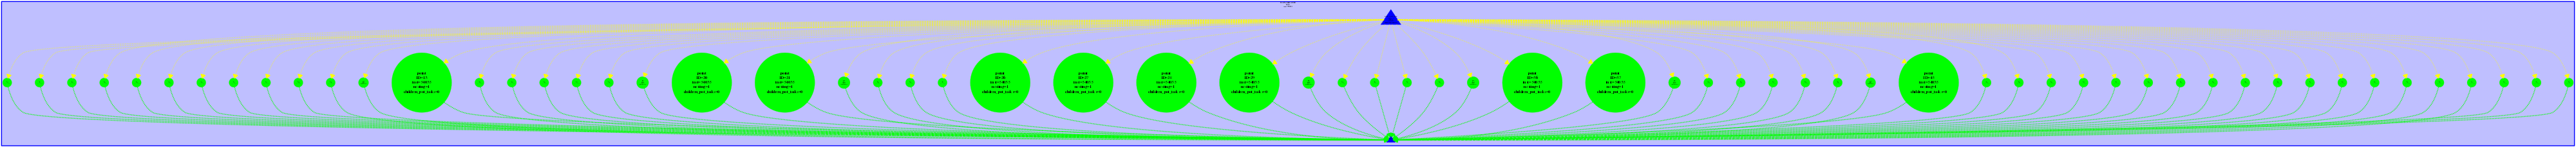
\includegraphics[scale=0.106]{./mandel-tar_point}
	\caption{Mandel-tar task decomposition graph using the point decomposition strategy.}
	\label{fig:mandel-tar-point}
\end{figure}

\begin{figure}[H]
	\centering
	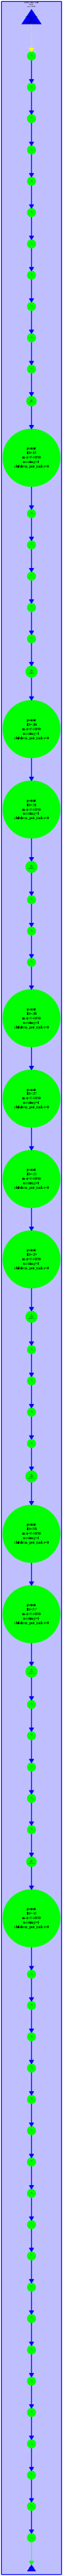
\includegraphics[scale=0.106]{./mandeld-tar_point}
	\caption{Mandeld-tar task decomposition graph using the point decomposition strategy.}
	\label{fig:mandeld-tar-point}
\end{figure}

This strategy will have more overhead of creation and termination of tasks than in the row strategy because it has to create more tasks. However, as a positive point the tasks are better distributed because if in a row there are many white areas, this work will not only be done by a single thread. Thus, it may end the execution earlier than in the row decomposition strategy.

\subsection{Row decomposition}

In this other strategy, a task corresponds with the computation of a whole row of the Mandelbrot set. This strategy only creates $row$ tasks.

In this case, the code is not the same as before. We changed the creation of the \textit{Tareador} tasks so that each time we enter a new row (second loop) a new task is created. The modified version of the code is shown below.

\begin{figure}[H]
\begin{lstlisting}
for (row = 0; row < height; ++row) {
	tareador_start_task("row");
	for (col = 0; col < width; ++col) {
		...
	}
	tareador_end_task("row");
}
\end{lstlisting}
\caption{Modified fragment of the \textit{mandel-tar.c} code.}
\label{code:mandeltarRow}
\end{figure}

Afterwards, we executed interactively mandel-tar and mandeld-tar again. We used the same size as before. Hence, the total number of tasks will be 8. The graphical results we got can be seen in figures \ref{fig:mandel-tar-row} and \ref{fig:mandeld-tar-row}.

\begin{figure}[H]
	\centering
	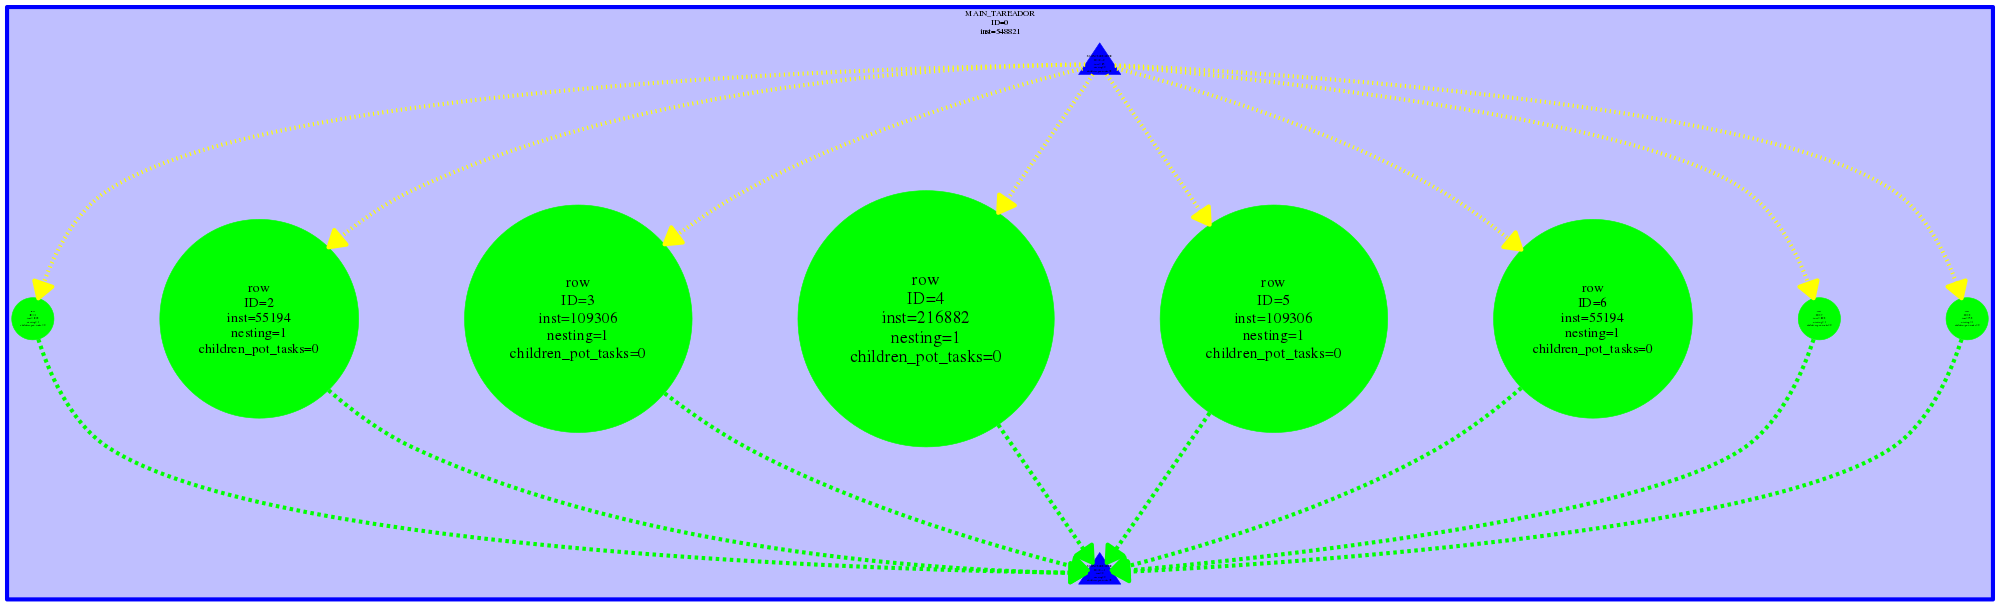
\includegraphics[scale=0.106]{./mandel-tar_row}
	\caption{Mandel-tar task decomposition graph using the row decomposition strategy.}
	\label{fig:mandel-tar-row}
\end{figure}

\begin{figure}[H]
	\centering
	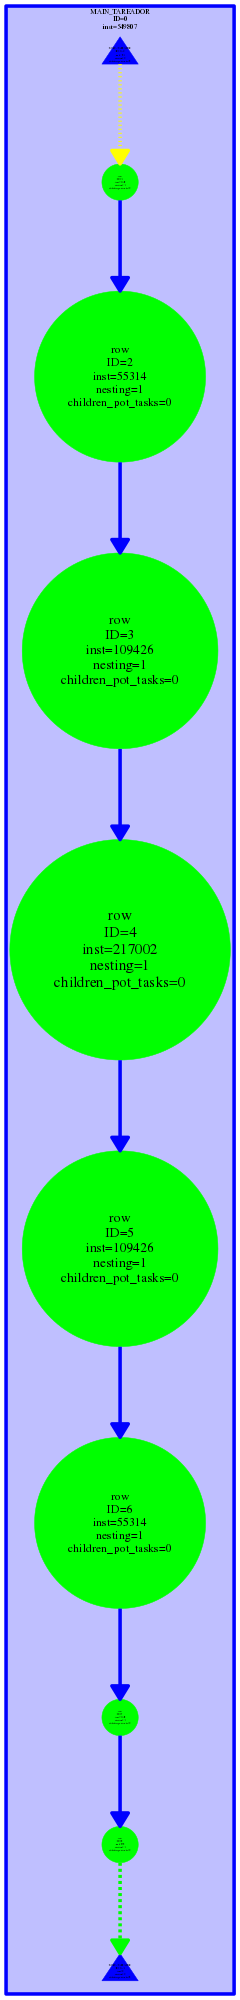
\includegraphics[scale=0.106]{./mandeld-tar_row}
	\caption{Mandeld-tar task decomposition graph using the row decomposition strategy.}
	\label{fig:mandeld-tar-row}
\end{figure}

In this strategy, the overhead time of creation and termination of tasks will be very small in comparison with the point strategy because it has to create less tasks. Nevertheless, it may happen that in a full row, all of its pixels must be white. In this case, it can happen that while other threads have finished their work, this other thread is still executing the row. Consequently, it is possible that the execution time may be bigger than in the point decomposition strategy.

\subsection{Characteristics of the TDG}

We saw in the previous sections that the execution of the mandel-tar has a very different task dependence graph than the execution of the mandeld-tar.

On the one hand, we can see that in mandel-tar every point is independent from the others. Consequently, we could parallelize that fragment of the code using OpenMP clauses.

On the other hand, in mandeld-tar we can see that all iterations have became sequential. In this situation, we do not gain anything by parallelizing the code, but we increase the execution time because of the overhead of creation and termination of tasks.

Using the \textit{Tareador} we could see which variable was responsible of creating those dependences. We did the following: Right Click into a task -$>$ Data View -$>$ Edges-out -$>$ Real Dependency. Figure \ref{fig:dependence_X11_COLOR_fake} shows the result we got.

\begin{figure}[H]
	\centering
	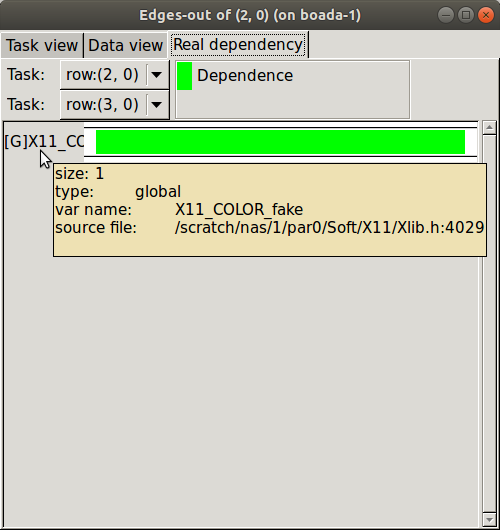
\includegraphics[scale=0.40]{./dependence_X11_COLOR_fake}
	\caption{Variable that provoques the dependences between tasks.}
	\label{fig:dependence_X11_COLOR_fake}
\end{figure}

We can see that there is only one variable that is causing all the dependences: X11\_COLOR\_fake. Observing the code, we noticed that the only difference between mandel-tar and mandeld-tar was a fragment of the code that was only executed in mode \_DISPLAY\_ (mandeld-tar):

\begin{figure}[H]
\begin{lstlisting}
#if _DISPLAY_
    /* Scale color and display point  */
    long color = (long) ((k-1) * scale_color) + min_color;
    if (setup_return == EXIT_SUCCESS) {
        XSetForeground (display, gc, color);
        XDrawPoint (display, win, gc, col, row);
    }
#else
    output[row][col]=k;
#endif
\end{lstlisting}
\caption{Fragment of the \textit{mandel-tar.c} code.}
\label{fig:display_code}
\end{figure}

Therefore, variable X11\_COLOR\_fake is used at least in one of the functions XSetForeground and XDrawPoint. We could protect this section of code in the parallel OpenMP code using the \textit{critical} clause to define a region of mutual exclusion where only one thread can be working at the same time.

\begin{figure}[H]
\begin{lstlisting}
#if _DISPLAY_
    /* Scale color and display point  */
    long color = (long) ((k-1) * scale_color) + min_color;
    
    #pragma omp critical
    if (setup_return == EXIT_SUCCESS) {
        XSetForeground (display, gc, color);
        XDrawPoint (display, win, gc, col, row);
    }
#else
    output[row][col]=k;
#endif
\end{lstlisting}
\caption{Fragment of the \textit{mandel-tar.c} code using the \textit{critical} clause to protect a fragment of the code.}
\label{fig:display_code}
\end{figure}

\section{Point decomposition in OpenMP}

In this section, we are going to explore different options in the OpenMP tasking model to express the Point decomposition for the Mandelbrot computation program. We will analyse the scalability and behaviour of these options.

\subsection{OpenMP Task Implementation}

The aim of this tasking model strategy is to create a task for each point. Figure \ref{code:task_implementation_point} show the OpenMP clauses we used to implement the task strategy (the code can be found in file \textit{mandel-omp-task-point.c} in codes folder).

\begin{figure}[H]
\begin{lstlisting}
for (int row = 0; row < height; ++row) {
	#pragma omp parallel
	#pragma omp single
    for (int col = 0; col < width; ++col) {
         #pragma omp task firstprivate(col)
         {
			...
			#pragma omp critical
	        if (setup_return == EXIT_SUCCESS) {
	        	XSetForeground (display, gc, color);
	        	XDrawPoint (display, win, gc, col, row);
	        }
			...
         }
     }
}
\end{lstlisting}
\caption{Fragment of the \textit{mandel-omp-task-point.c} code showing the OpenMP clauses to implement the task strategy.}
\label{code:task_implementation_point}
\end{figure}

For every row, only one thread is creating all the tasks and inserting them into a pool of tasks, while the other threads are taking tasks from the pool and executing them. Nevertheless, the "role" of creating tasks changes for every row. Thus, each iteration of the col loop will be executed as an independent task. The firstprivate clause is used in order to avoid problems of data races\footnote{We have not used the private clause because it initializes the variable with a random value, and we wanted the real value of the variable (iteration).}. Finally, the critical clause is used to honour the dependences we detected for the graphical version in the previous section. However, this section of the code will not be called since we will not execute the graphical version (only mandel-tar).

The following figure shows the execution flow of the program using the \textit{Paraver} tool.

\begin{figure}[H]
	\centering
	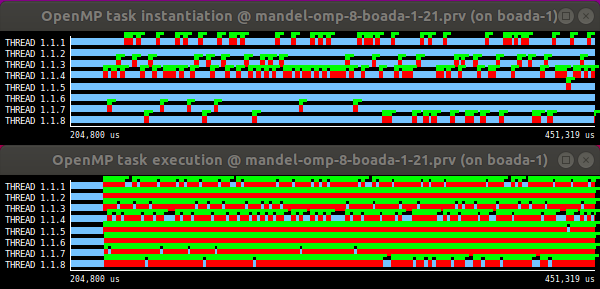
\includegraphics[scale=0.40]{./S2_OMP_tasks}
	\caption{Zoomed part of the execution flow using the task strategy.}
	\label{fig:S2_OMP_tasks}
\end{figure}

We can observe the effect of the single clause. In the upper part (task instantiation) only one thread is creating the tasks and inserting them in the task pool. In the bottom part (task execution) we can see that the other threads execute the tasks as they are put in the pool. The role of the task creator changes every time we finish a row.

In total, there are 640000 tasks created and executed. This is because the image has size $800 \times 800$. We have seen this using the "OMP\_parallel\_functions.cfg" and "OMP\_state\_profile.cfg" configurations (figure \ref{fig:S2_OMP_tasks_table}). The parallel construct is executed 800 times (figure \ref{fig:mandel-omp-21-parallel}), the number of rows. Finally, the single worksharing construct is executed 800 times for each thread (figure \ref{fig:mandel-omp-21-single}). Thus, the single clause is executed 6400 times ($rows \times threads$). All threads will execute the single line but only one will "gain". This thread will be responsible for creating the tasks of that row.

\begin{figure}[H]
\centering
\begin{minipage}[t]{0.4\linewidth}
  \centering
  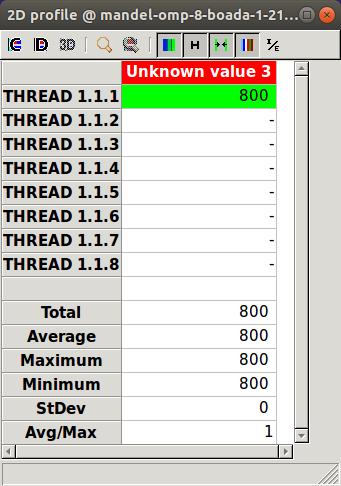
\includegraphics[scale=0.40]{./mandel-omp-21-parallel}
  \caption{Table with the total number of times \#pragma omp parallel has been called by each thread.}
  \label{fig:mandel-omp-21-parallel}
\end{minipage}%
\hspace{0.5cm}
\begin{minipage}[t]{0.4\linewidth}
  \centering
  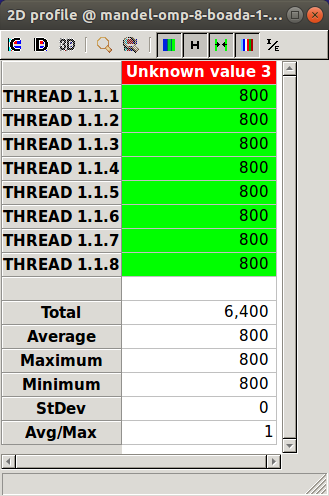
\includegraphics[scale=0.40]{./mandel-omp-21-single}
  \caption{Table with the total number of times \#pragma omp single has been called by each thread.}
  \label{fig:mandel-omp-21-single}
\end{minipage}
\end{figure}

\begin{figure}[H]
	\centering
	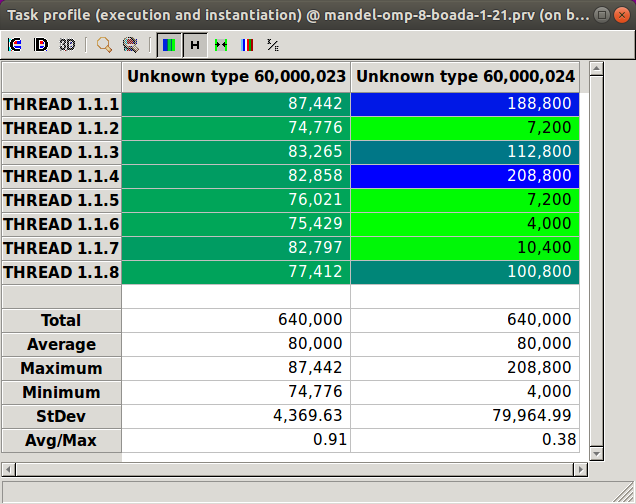
\includegraphics[scale=0.40]{./S2_OMP_tasks_table}
	\caption{Table with the number of executed tasks in the left column and the number of created tasks in the right column.}
	\label{fig:S2_OMP_tasks_table}
\end{figure}

Finally, figures \ref{fig:mandel-omp-10000-strong-21-time} and \ref{fig:mandel-omp-10000-strong-21-speedup} show the time and speedup plots.

\begin{figure}[H]
\centering
\begin{minipage}[b]{0.4\linewidth}
  \centering
  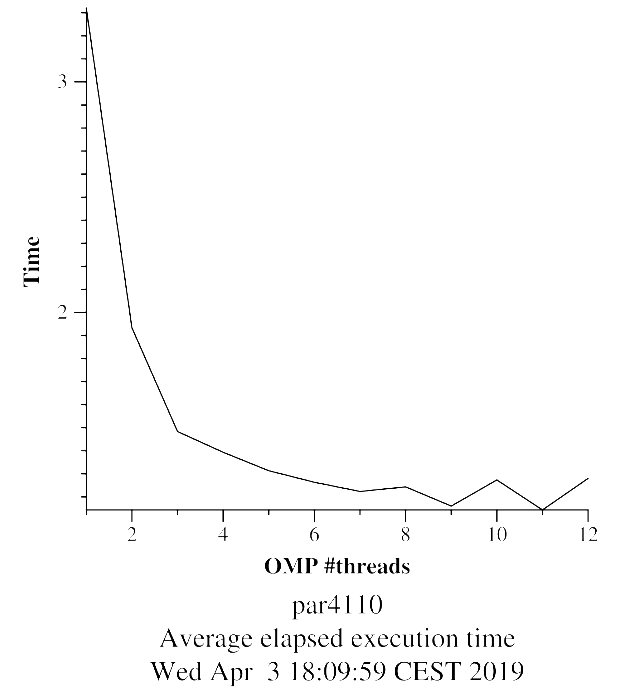
\includegraphics[scale=0.5]{./mandel-omp-10000-strong-21-time}
  \caption{Execution time plot varying the number of threads.}
  \label{fig:mandel-omp-10000-strong-21-time}
\end{minipage}%
\hspace{0.5cm}
\begin{minipage}[b]{0.4\linewidth}
  \centering
  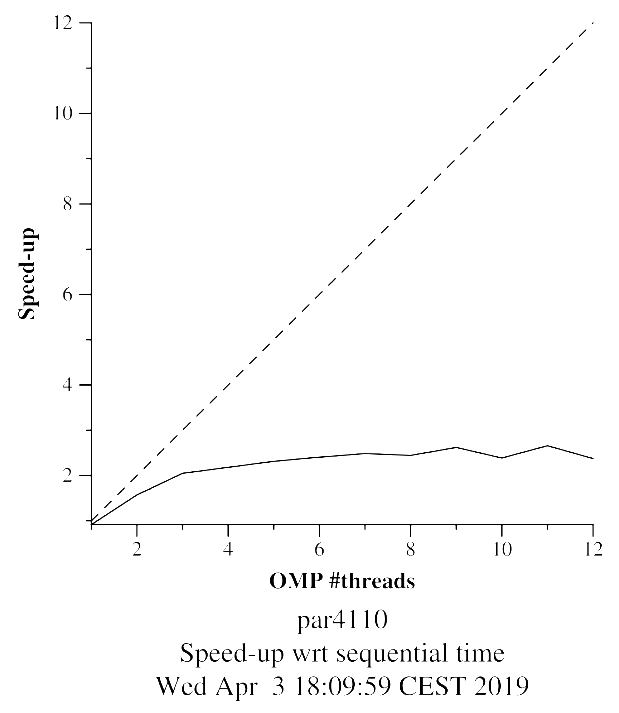
\includegraphics[scale=0.5]{./mandel-omp-10000-strong-21-speedup}
  \caption{Speedup plot varying the number of threads.}
  \label{fig:mandel-omp-10000-strong-21-speedup}
\end{minipage}
\end{figure}

In the first plot, the execution time is reduced as we increase the number of threads until the time stays constant. However, we think that if we increase a lot the number of threads, the execution time would end up increasing because of the overheads.

On the other hand, in the second plot the speedup increases a lot with 2-4 threads but ends up constant as we increase the number of threads.

Finally, the scalability is not appropiate because the speedup stays at 2 when we are using a big number of threads.

\subsubsection{OpenMP Taskwait Variant}

In this variant of the previous code, only one thread (the one that gets access to the single region), traverses all iterations of the row and col loops, generating a task for each iteration of the innermost loop (point). To do it, we have introduced "\#pragma omp taskwait" at the end of each iteration of a row. Consequently, the creator thread must wait until all tasks for a row finish. After that, the thread will advance one iteration of the row loop and generate a new bunch of tasks. This new version of the code can be found in \textit{mandel-omp-task-point-taskwait.c}.

\begin{figure}[H]
\begin{lstlisting}
#pragma omp parallel
#pragma omp single
for (int row = 0; row < height; ++row) {
	for (int col = 0; col < width; ++col) {
		#pragma omp task firstprivate(row, col)
		{
			...
		}
	}
	#pragma omp taskwait // waiting point for all child tasks
}
\end{lstlisting}
\caption{Fragment of the \textit{mandel-omp-task-point-taskwait.c} code showing the OpenMP clauses to implement the task strategy with the taskwait variant.}
\label{code:task_implementation_point_taskwait}
\end{figure}

We can clearly see in figures \ref{fig:S2_OMP_tasks_22}, \ref{fig:S2_OMP_tasks_22_zoom} and \ref{fig:S2_OMP_tasks_table_22} that the only thread that is creating tasks is the thread 0. Moreover, in the zoomed figure we can observe that every time it creates some tasks, then it has to wait a little bit until it can create tasks again. This is because of the taskwait clause we added at the end of the outermost loop. Thread 0 will create all the tasks for a unique row and will wait until all these tasks terminate.

\begin{figure}[H]
\begin{minipage}[t]{0.5\linewidth}
  \centering
  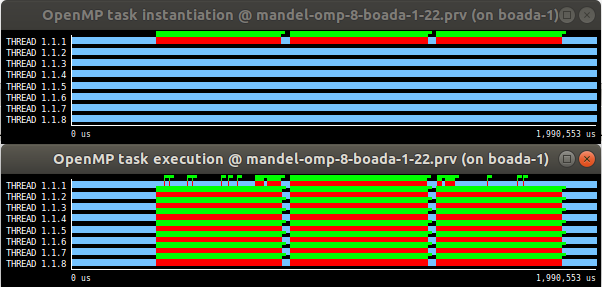
\includegraphics[scale=0.345]{./S2_OMP_tasks_22}
  \caption{Execution flow using the taskwait strategy.}
  \label{fig:S2_OMP_tasks_22}
\end{minipage}%
\hspace{0cm}
\begin{minipage}[t]{0.5\linewidth}
  \centering
  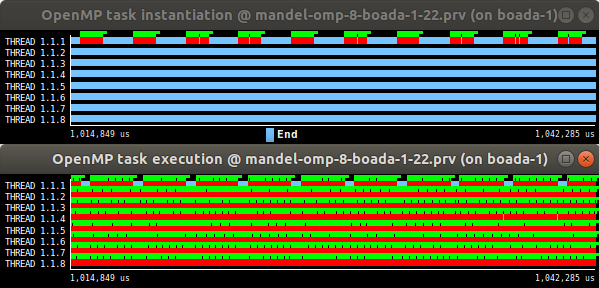
\includegraphics[scale=0.345]{./S2_OMP_tasks_22_zoom}
  \caption{Zoomed part of Figure \ref{fig:S2_OMP_tasks_22}.}
  \label{fig:S2_OMP_tasks_22_zoom}
\end{minipage}
\end{figure}


The number of created and executed tasks is still 640000 as we have not modified the size of the image (figure \ref{fig:S2_OMP_tasks_table_22}). Nevertheless, the number of calls to parallel is 1 (figure \ref{fig:mandel-omp-22-parallel}), and the number of calls to the single worksharing construct is now 8 (figure \ref{fig:mandel-omp-22-single}), the number of threads. Besides, the taskwait clause will be executed 800 times (number of rows). The granularity is the same than before. Each task has exactly one iteration of the innermost for loop.

\begin{figure}[H]
\centering
\begin{minipage}[t]{0.4\linewidth}
  \centering
  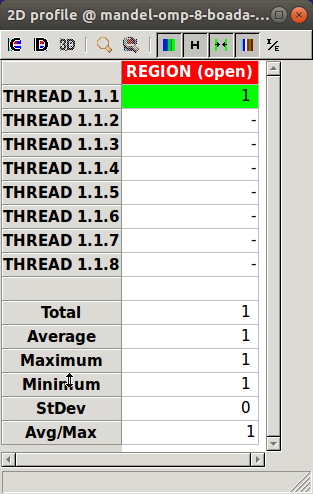
\includegraphics[scale=0.40]{./mandel-omp-22-parallel}
  \caption{Table with the total number of times \#pragma omp parallel has been called by each thread.}
  \label{fig:mandel-omp-22-parallel}
\end{minipage}%
\hspace{0.5cm}
\begin{minipage}[t]{0.4\linewidth}
  \centering
  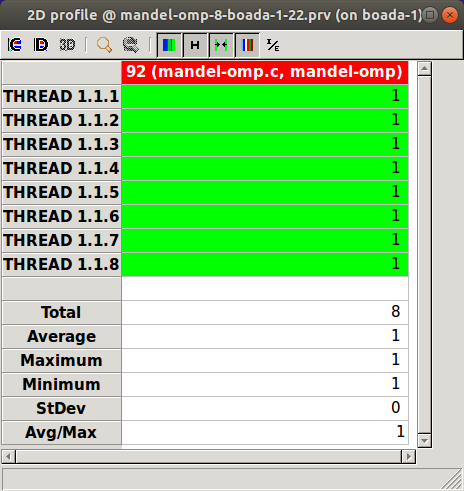
\includegraphics[scale=0.40]{./mandel-omp-22-single}
  \caption{Table with the total number of times \#pragma omp single has been called by each thread.}
  \label{fig:mandel-omp-22-single}
\end{minipage}
\end{figure}

\begin{figure}[H]
	\centering
	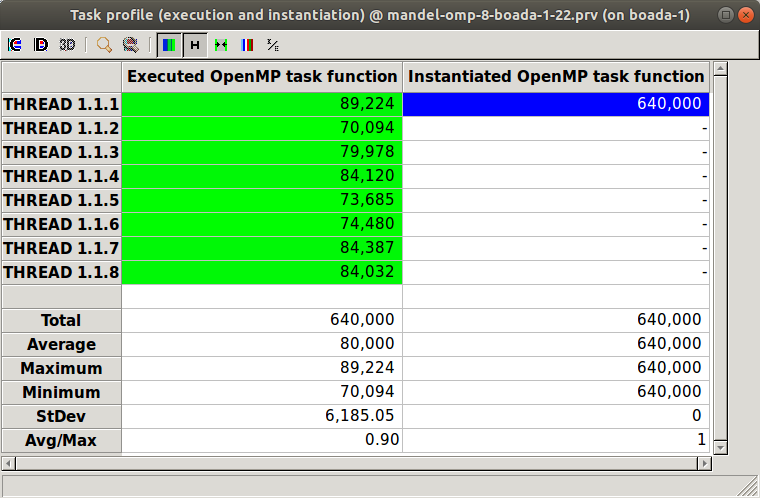
\includegraphics[scale=0.40]{./S2_OMP_tasks_table_22}
	\caption{Table with the number of executed tasks in the left column and the number of created tasks in the right column.}
	\label{fig:S2_OMP_tasks_table_22}
\end{figure}

From here, as we will not change the \#pragma omp parallel and \#pragma omp single anymore, figures \ref{fig:mandel-omp-22-parallel} and \ref{fig:mandel-omp-22-single} will be the same for the following variants and new implementations.

Figures \ref{fig:mandel-omp-10000-strong-22-time} and \ref{fig:mandel-omp-10000-strong-22-speedup} show again the time and speedup plots. We have not noticed any significant difference between these plots and the plots of the previous section.

\begin{figure}[H]
\centering
\begin{minipage}[b]{0.4\linewidth}
  \centering
  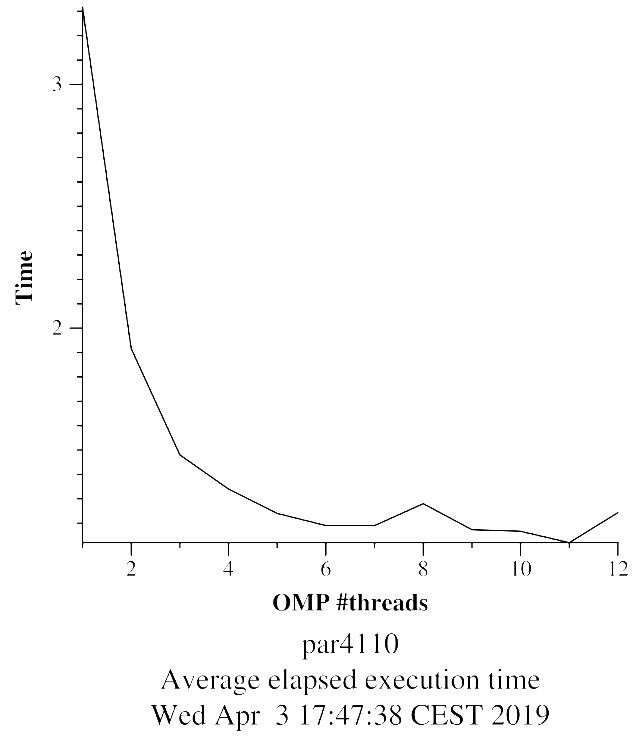
\includegraphics[scale=0.5]{./mandel-omp-10000-strong-22-time}
  \caption{Execution time plot varying the number of threads.}
  \label{fig:mandel-omp-10000-strong-22-time}
\end{minipage}%
\hspace{0.5cm}
\begin{minipage}[b]{0.4\linewidth}
  \centering
  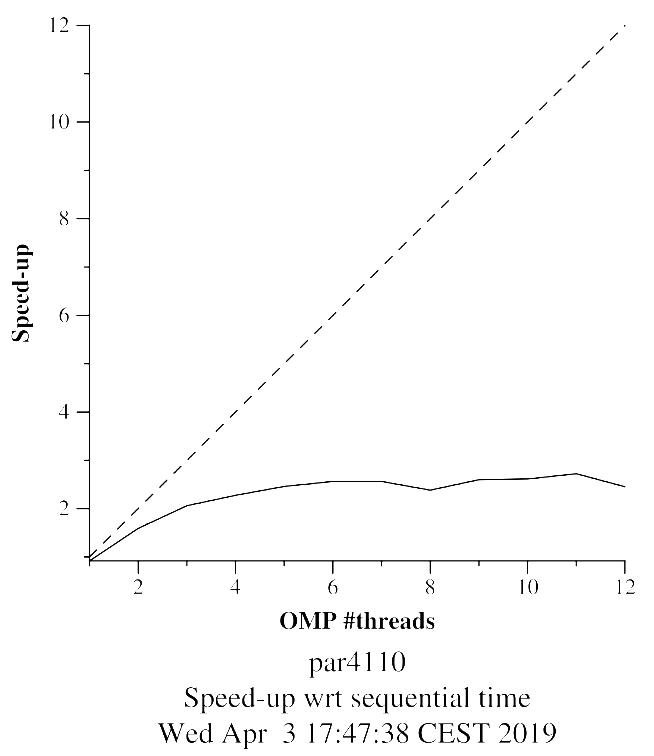
\includegraphics[scale=0.5]{./mandel-omp-10000-strong-22-speedup}
  \caption{Speedup plot varying the number of threads.}
  \label{fig:mandel-omp-10000-strong-22-speedup}
\end{minipage}
\end{figure}

\paragraph{The Taskwait Clause}

\hfill

In reality, the taskwait clause is not necessary because tasks do not have any dependence between them. We saw in section \ref{sec:tareador} that the mandel-tar binary does not produce any kind of dependence between tasks. Thus, we can create and execute all tasks without having to wait until some of them terminate. The modified version of the code can be found in the file \textit{mandel-omp-task-point-taskwait-without.c}.

In order to see the differences with respect to the version with the taskwait clause, we have repeated the evaluation of scalability and tracing. The results are shown below.

\begin{figure}[H]

\begin{minipage}[t]{0.5\linewidth}
  \centering
  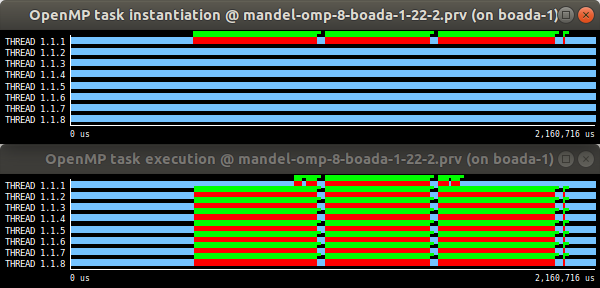
\includegraphics[scale=0.345]{./S2_OMP_tasks_22_2}
  \caption{Execution flow using the taskwait strategy without the barrier.}
  \label{fig:S2_OMP_tasks_22_2}
\end{minipage}%
\hspace{0cm}
\begin{minipage}[t]{0.5\linewidth}
  \centering
  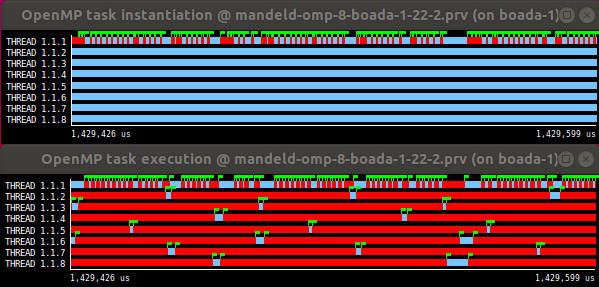
\includegraphics[scale=0.345]{./S2_OMP_tasks_22_2_zoom}
  \caption{Zoomed part of Figure \ref{fig:S2_OMP_tasks_22_2}.}
  \label{fig:S2_OMP_tasks_22_2_zoom}
\end{minipage}
\end{figure}

The number of tasks created/executed has not changed because we have not touched the task clause or the parallel and single clauses. However, as we have deleted the taskwait clause, now the creator thread (thread 0 in our case) does not have to wait until the tasks of the same row terminate. Consequently, it can create all possible tasks of the program at the same time. Nevertheless, we see in figures \ref{fig:S2_OMP_tasks_22_2} and \ref{fig:S2_OMP_tasks_22_2_zoom} that this is not happening as expected.

We though that thread 0 would create all possible tasks and then execute the remaining tasks inside the task pool. What is happening is that this thread creates some tasks, then stops the task generation, then executes some taks, and then proceeds generating new tasks. After reasoning about this, we have concluded that the task pool that OpenMP has is limited, it has a maximum number of threads inside the pool. As a consequence, when thread 0 reaches this limit it has to stop creating tasks, so it begins to execute the created tasks until the total number of tasks inside the pool is reduced. Afterwards, it begins to create tasks again.

On the other hand, we can see that the scalability plots (time and speedup) have improved a bit even though it is not a significative change.

\begin{figure}[H]
\centering
\begin{minipage}[b]{0.4\linewidth}
  \centering
  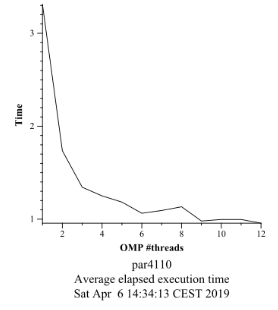
\includegraphics[scale=0.95]{./mandel-omp-10000-strong-22-2-time}
  \caption{Execution time plot varying the number of threads.}
  \label{fig:mandel-omp-10000-strong-22-2-time}
\end{minipage}%
\hspace{0.5cm}
\begin{minipage}[b]{0.4\linewidth}
  \centering
  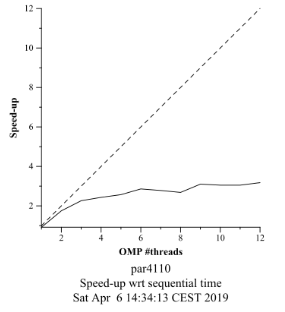
\includegraphics[scale=0.95]{./mandel-omp-10000-strong-22-2-speedup}
  \caption{Speedup plot varying the number of threads.}
  \label{fig:mandel-omp-10000-strong-22-2-speedup}
\end{minipage}
\end{figure}

To sum up, we can delete the taskwait clause because it is not necessary for mandel-tar. This change improves a little bit the performance of the execution. Moreover, without this clause the creator thread has to stop generating tasks because it reaches the maximum limit of the pool. Thus, it will be changing from creating to executing and vice versa very often.

\subsubsection{OpenMP Taskgroup Variant}

In this other variant, we define a region in the program where the thread will wait for the termination of all descendant (not only child) tasks. Figure \ref{code:task_implementation_point_taskgroup} shows a section of the modified code that can be found in file \textit{mandel-omp-task-point-taskgroup.c} inside the codes directory. Now, the tasks of the same row are generated without any specific order. However, the creator thread has to wait until all the tasks of the same row terminate.

\begin{figure}[H]
\begin{lstlisting}
#pragma omp parallel
#pragma omp single
for (int row = 0; row < height; ++row) {
	#pragma omp taskgroup
	{
		for (int col = 0; col < width; ++col) {
        	#pragma omp task firstprivate(row, col)
        	{
        		...
			}
		}
	}
}
\end{lstlisting}
\caption{Fragment of the \textit{mandel-omp-task-point-taskgroup.c} code showing the OpenMP clauses to implement the task strategy with the taskgroup variant.}
\label{code:task_implementation_point_taskgroup}
\end{figure}

In the execution flow we obtained with \textit{Paraver} we can see that there is no differenece at all with respect to the execution flow of the previous section. This is because in reality the taskgroup clause does not have descendants of its childs. As a consequence, it does the same effect than using the taskwait clause.

\begin{figure}[H]
\begin{minipage}[t]{0.5\linewidth}
  \centering
  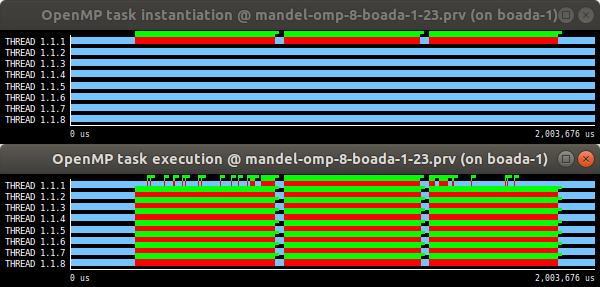
\includegraphics[scale=0.345]{./S2_OMP_tasks_23}
  \caption{Execution flow using the taskwait strategy without the barrier.}
  \label{fig:S2_OMP_tasks_23}
\end{minipage}%
\hspace{0cm}
\begin{minipage}[t]{0.5\linewidth}
  \centering
  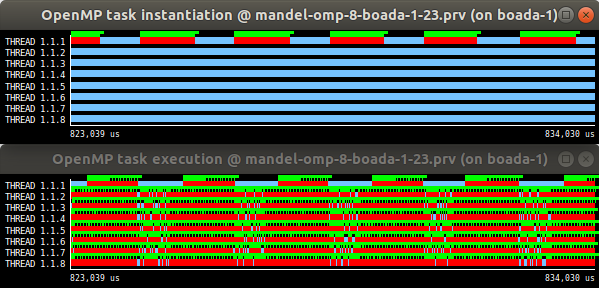
\includegraphics[scale=0.345]{./S2_OMP_tasks_23_zoom}
  \caption{Zoomed part of Figure \ref{fig:S2_OMP_tasks_23}.}
  \label{fig:S2_OMP_tasks_23_zoom}
\end{minipage}
\end{figure}

The number of created tasks is the same (640000). Moreover, the number of calls to parallel and the single worksharing contruct is the same (1 and 8 respectively). The only difference is that in this variant the taskgroup clause is executed 800 times (number of rows).

\begin{figure}[H]
	\centering
	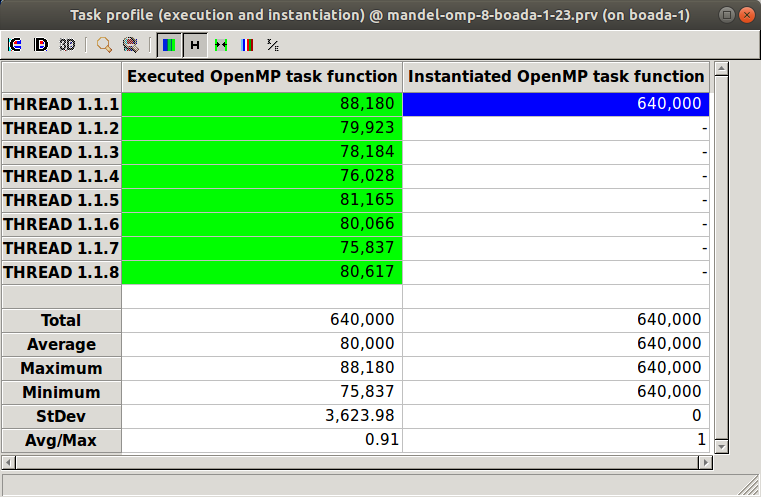
\includegraphics[scale=0.40]{./S2_OMP_tasks_table_23}
	\caption{Table with the number of executed tasks in the left column and the number of created tasks in the right column.}
	\label{fig:S2_OMP_tasks_table_23}
\end{figure}

Figures \ref{fig:mandel-omp-10000-strong-23-time} and \ref{fig:mandel-omp-10000-strong-23-speedup} show again the time and speedup plots. We have not noticed any significant difference between these plots and the plots of the two previous sections.

\begin{figure}[H]
\centering
\begin{minipage}[b]{0.4\linewidth}
  \centering
  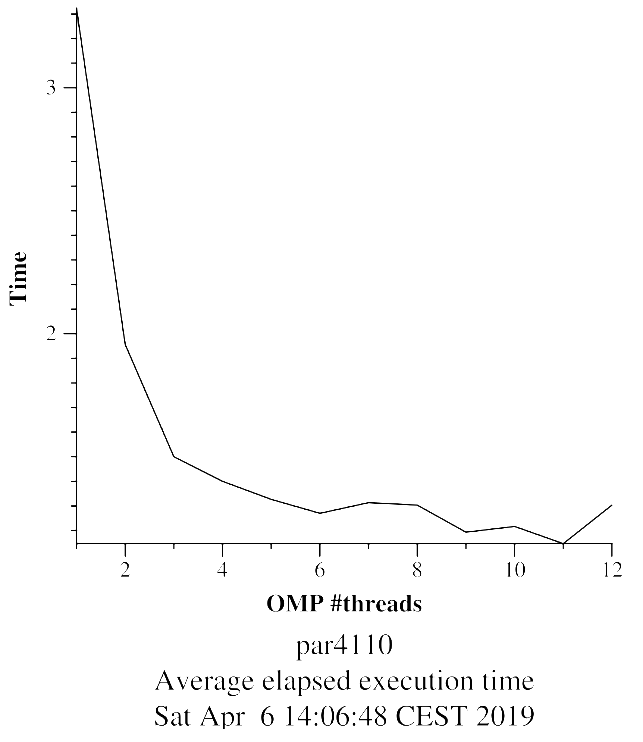
\includegraphics[scale=0.5]{./mandel-omp-10000-strong-23-time}
  \caption{Execution time plot varying the number of threads.}
  \label{fig:mandel-omp-10000-strong-23-time}
\end{minipage}%
\hspace{0.5cm}
\begin{minipage}[b]{0.4\linewidth}
  \centering
  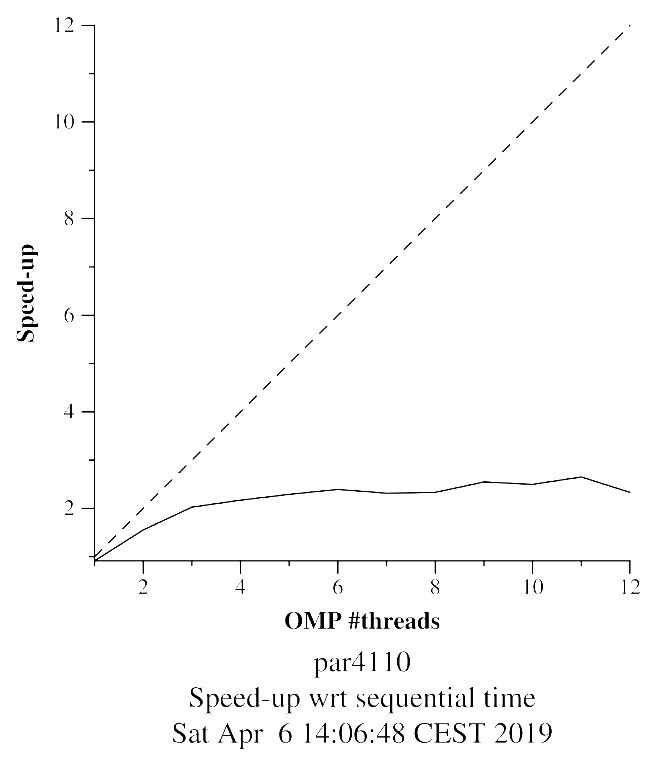
\includegraphics[scale=0.5]{./mandel-omp-10000-strong-23-speedup}
  \caption{Speedup plot varying the number of threads.}
  \label{fig:mandel-omp-10000-strong-23-speedup}
\end{minipage}
\end{figure}

\subsection{OpenMP Taskloop Implementation}

In this new strategy, the taskloop clause is used. It generates tasks out of its iterations of a for loop, allowing to better control the number of tasks generated or their granularity (num\_tasks or grainsize). This version of the code can be found in the file \textit{mandel-omp-task-point-taskloop-800}.

\begin{figure}[H]
\begin{lstlisting}
#pragma omp parallel
#pragma omp single
for (int row = 0; row < height; ++row) {
	#pragma omp taskloop firstprivate(row) num_tasks(800)
    for (int col = 0; col < width; ++col) {
    	...
    }
}
\end{lstlisting}
\caption{Fragment of the \textit{mandel-omp-task-point-taskloop-800.c} code showing the OpenMP clauses to implement the task strategy with the taskloop variant.}
\label{code:task_implementation_point_taskloop_800}
\end{figure}

If we create 800 tasks of the mostinner loop, in reality we are executing an equivalent version of the second task version we analysed. In order to analyse the performance of this strategy we will use the traces generated with \textit{Paraver} and using the appropiate configuration files.

\begin{figure}[H]
\begin{minipage}[t]{0.48\linewidth}
  \centering
  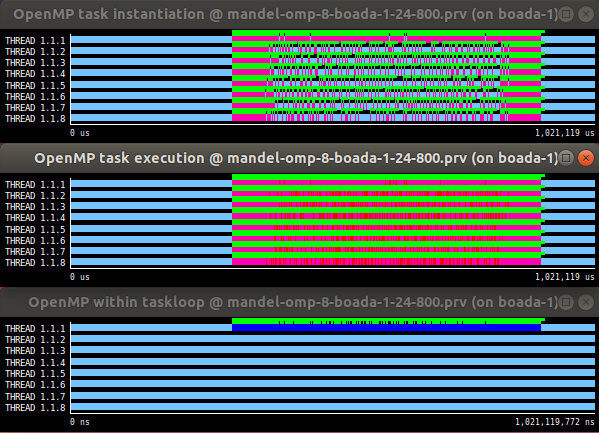
\includegraphics[scale=0.35]{./S2_OMP_tasks_24_800}
  \caption{Execution flow of using the taskloop strategy and 800 tasks for each row.}
  \label{fig:S2_OMP_tasks_24_800}
\end{minipage}%
\hspace{0.5cm}
\begin{minipage}[t]{0.48\linewidth}
  \centering
  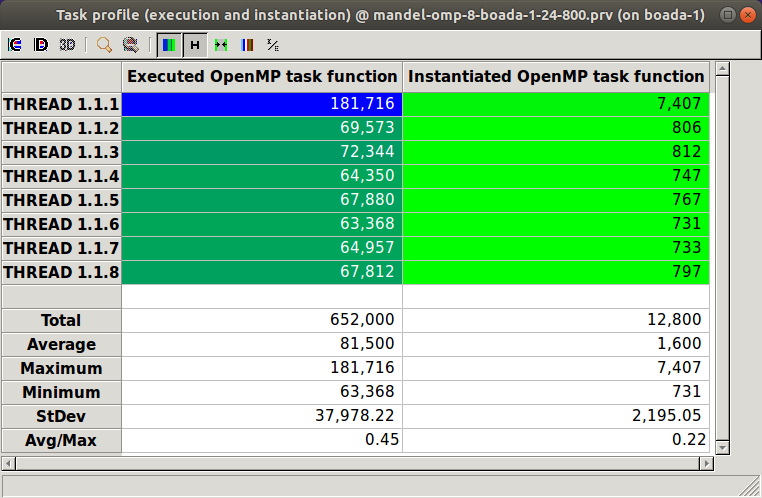
\includegraphics[scale=0.3]{./S2_OMP_tasks_24_800_table}
  \caption{Table with the number of executed tasks in the left column and the number of created tasks in the right column.}
  \label{fig:S2_OMP_tasks_24_800_table}
\end{minipage}
\end{figure}

First of all, we can see something strange in figure \ref{fig:S2_OMP_tasks_24_800} in the instatiation part. In the first moment all threads create a lot of tasks, then only thread 0 is the one creating most of the tasks, and then all threads create again all the tasks. The reasoning about this effect will be done in the next section, when comparing the results with another 2 traces.

On the other hand, in figure \ref{fig:S2_OMP_tasks_24_800_table} we can see that there are created more than 640000 tasks, the expected number. The reason we got when asking to the professor was that when using the \textit{Paraver} and the taskloop, there are created some metatasks to evaluate some things. Thus, the number of created tasks is increased a bit.

\subsubsection{The Nogroup Clause}

The taskloop construct has an implicit task barrier (taskgroup) at the end. This is causing the effect of a taskwait clause. As we reasoned before about that we could delete the taskwait clause because there are no dependences between tasks, we can do the same with the taskgroup clause. To do it, the taskloop construct accepts a nogroup clause that eliminates this implicit barrier.

Now, we will explore how this new version behaves in terms of performance when using 8 threads and for different task granularities (800, 400, 200, 100, 50, 25, 10, 5, 2 and 1 tasks). All versions of the codes can be found in files \textit{mandel-omp-task-point-taskloop-\{granularity\}-nogroup}.

\begin{figure}[H]
\begin{minipage}[t]{0.48\linewidth}
  \centering
  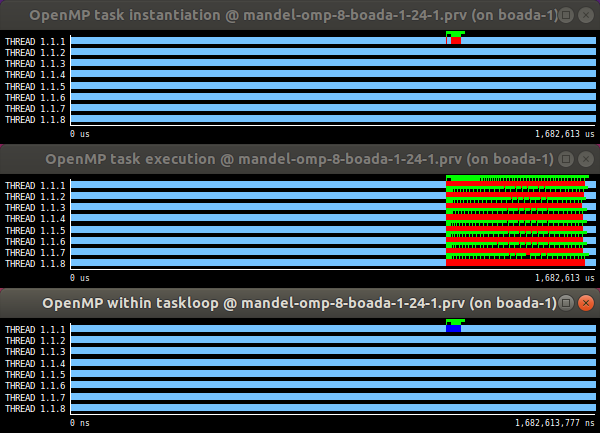
\includegraphics[scale=0.35]{./S2_OMP_tasks_24_1}
  \caption{Execution flow of using the taskloop strategy and 1 task for each row.}
  \label{fig:S2_OMP_tasks_24_1}
\end{minipage}%
\hspace{0.5cm}
\begin{minipage}[t]{0.48\linewidth}
  \centering
  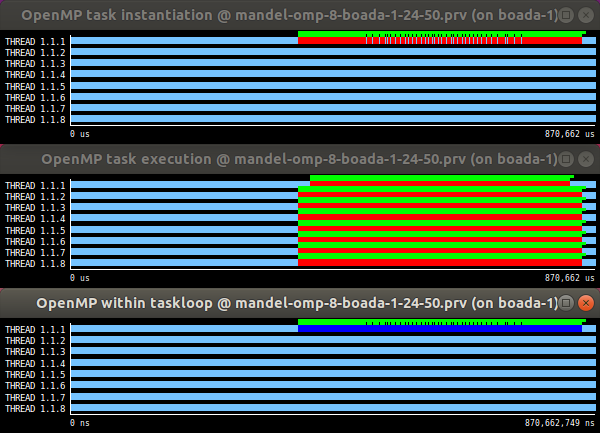
\includegraphics[scale=0.35]{./S2_OMP_tasks_24_50}
  \caption{Execution flow of using the taskloop strategy and 50 tasks for each row.}
  \label{fig:S2_OMP_tasks_24_50}
\end{minipage}
\end{figure}

In the previous traces we can observe multiple things. Firstly, the time expended creating tasks is reduced as we increase the granularity. It is common sense, if we create less tasks per row, we will expend less time doing it (thanks to the nogroup clause). Moreover, the execution time of the parallel part is also reduced with a smaller number of tasks. We think that this happen because there will be less overhead of creation, synchronization and termination and while some tasks execute the longer tasks, the rest will continue executing the other ones.

Secondly, we can see in figure \ref{fig:S2_OMP_tasks_24_800} a different behaviour with respect to figures \ref{fig:S2_OMP_tasks_24_1} and \ref{fig:S2_OMP_tasks_24_50}. All threads are creating tasks whereas in the other 2 traces only thread 0 is the one creating tasks.

Our conclusion is that in the version with number of tasks 800 threads end faster the upper, left and right parts of the non-created image because there are no white parts. Hence, as we have the nogroup clause and there are no more tasks inside the pool, they can create tasks too. However, in the middle of the image, as there are more white pixels, threads expend more time executing the task, so in this part they will create less tasks and thread 0 will be responsible for creating the biggest part of tasks. As we decrease the total number of tasks, threads will do more instructions per task. Thus, they will not have time to create tasks and only thread 0 will be responsible for creating all the tasks (from number of tasks 100 down, only thread 0 is creating the tasks).

The following plots are the scalability plots using the same implementation but varying the number of tasks per row. They are only a part of all. The rest of the plots can be found in section \ref{sec:point_taskloop_scalability_plots}.

\begin{figure}[H]
\begin{minipage}[t]{0.48\linewidth}
  \centering
  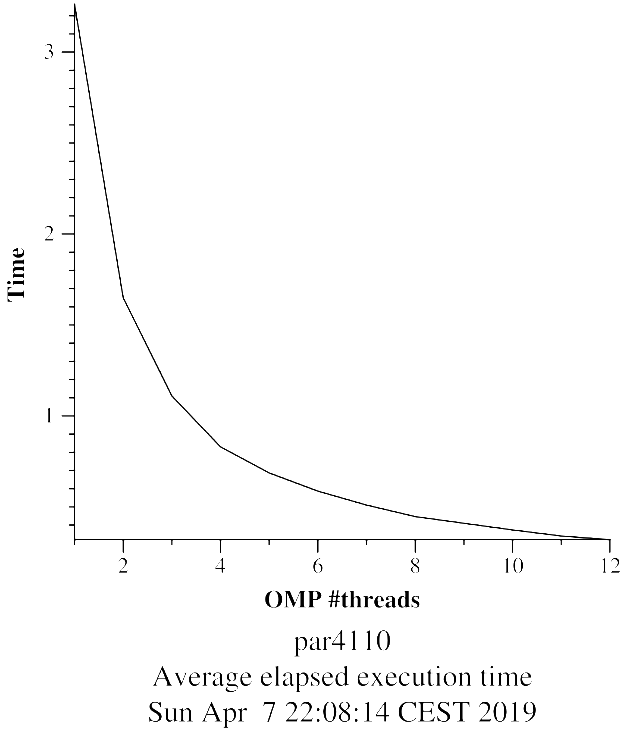
\includegraphics[scale=0.5]{./mandel-omp-10000-strong-omp-24-1-time}
  \caption{Time plot varying the number of threads and using 1 task.}
  \label{fig:mandel-omp-10000-strong-omp-24-1-time}
\end{minipage}%
\hspace{0.5cm}
\begin{minipage}[t]{0.48\linewidth}
  \centering
  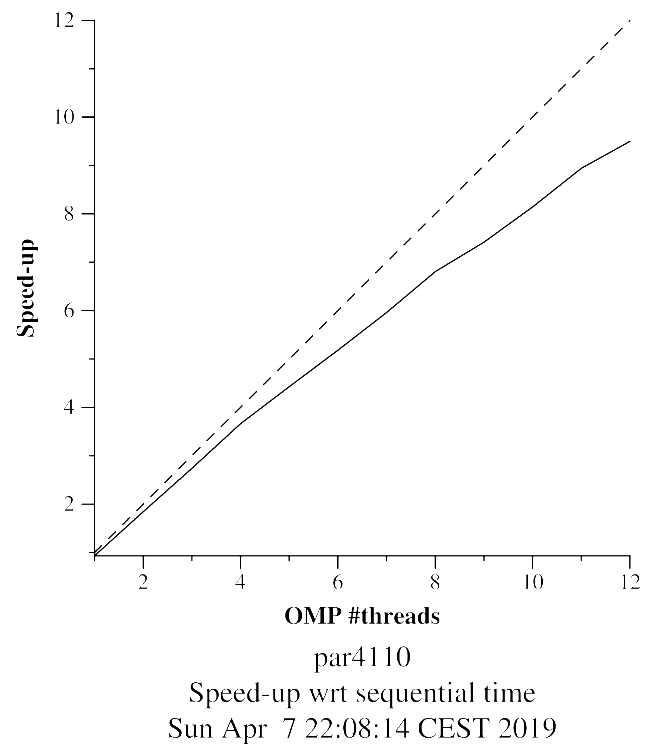
\includegraphics[scale=0.5]{./mandel-omp-10000-strong-omp-24-1-speedup}
  \caption{Speedup plot varying the number of threads and using 1 task.}
  \label{fig:mandel-omp-10000-strong-omp-24-1-speedup}
\end{minipage}
\end{figure}

\begin{figure}[H]
\begin{minipage}[t]{0.48\linewidth}
  \centering
  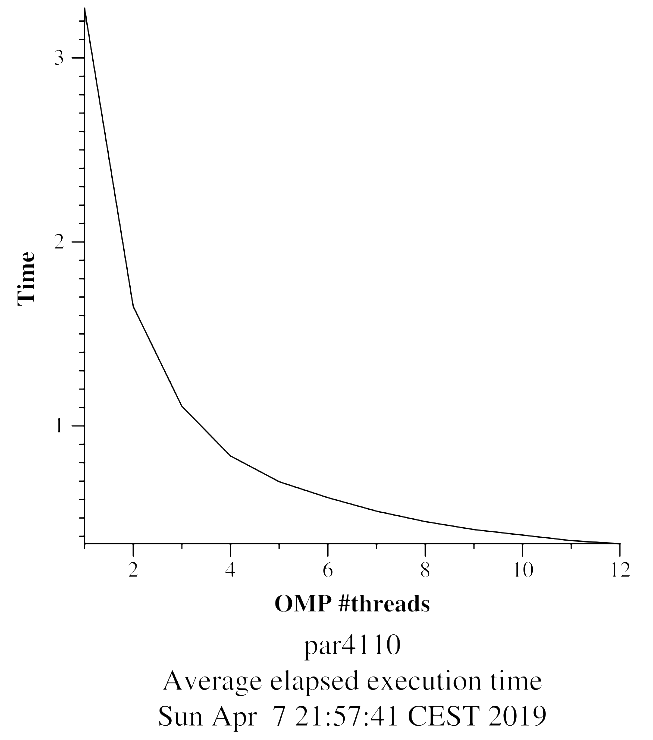
\includegraphics[scale=0.5]{./mandel-omp-10000-strong-omp-24-50-time}
  \caption{Time plot varying the number of threads and using 50 tasks.}
  \label{fig:mandel-omp-10000-strong-omp-24-50-time}
\end{minipage}%
\hspace{0.5cm}
\begin{minipage}[t]{0.48\linewidth}
  \centering
  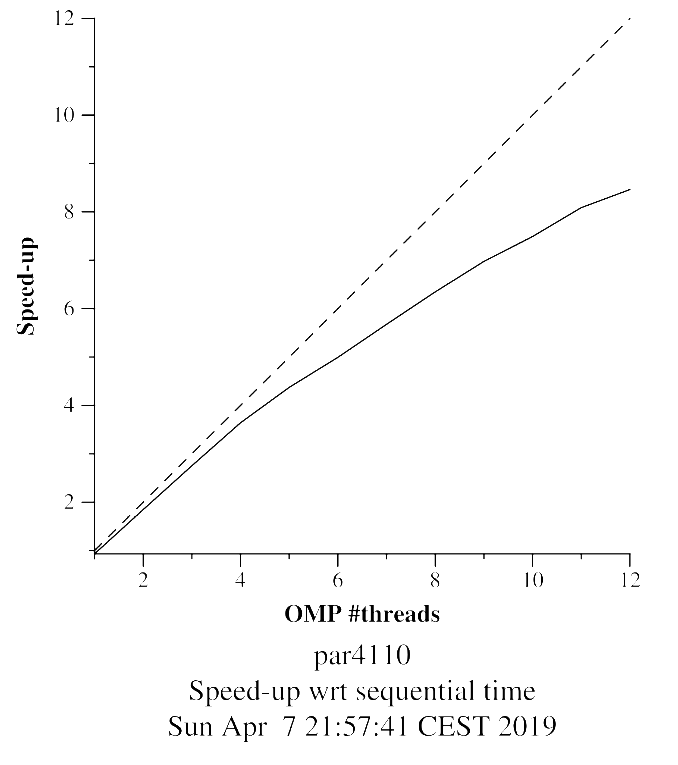
\includegraphics[scale=0.5]{./mandel-omp-10000-strong-omp-24-50-speedup}
  \caption{Speedup plot varying the number of threads and using 50 tasks.}
  \label{fig:mandel-omp-10000-strong-omp-24-50-speedup}
\end{minipage}
\end{figure}

\begin{figure}[H]
\begin{minipage}[t]{0.48\linewidth}
  \centering
  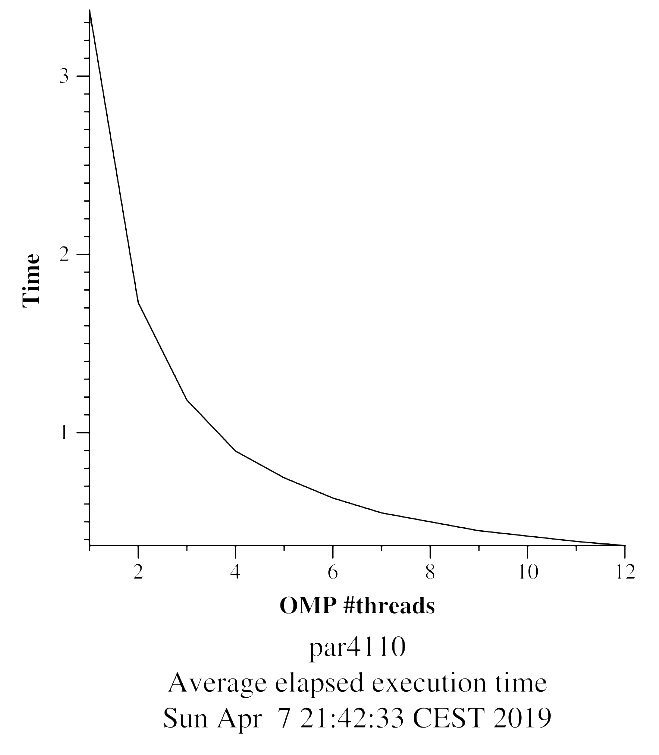
\includegraphics[scale=0.5]{./mandel-omp-10000-strong-omp-24-800-time}
  \caption{Time plot varying the number of threads and using 800 tasks.}
  \label{fig:mandel-omp-10000-strong-omp-24-800-time}
\end{minipage}%
\hspace{0.5cm}
\begin{minipage}[t]{0.48\linewidth}
  \centering
  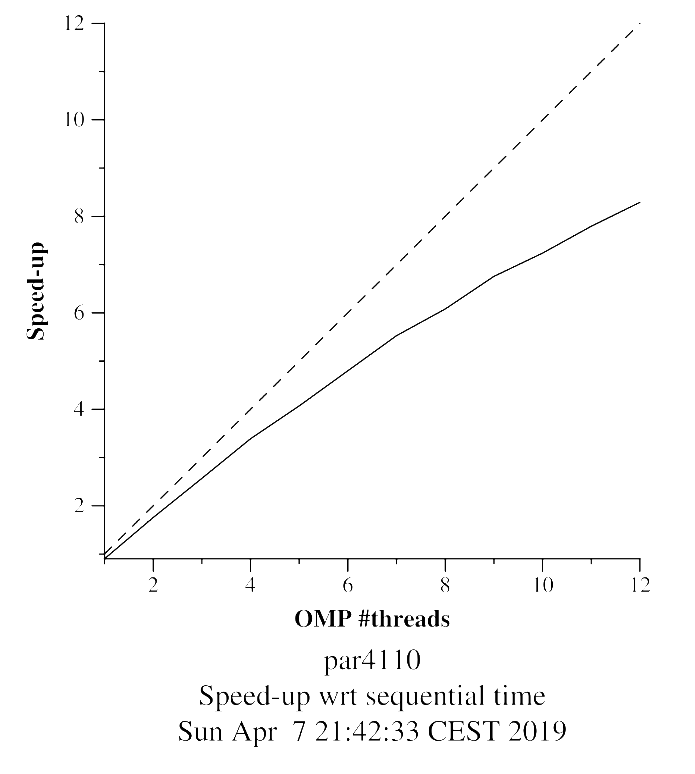
\includegraphics[scale=0.5]{./mandel-omp-10000-strong-omp-24-800-speedup}
  \caption{Speedup plot varying the number of threads and using 800 tasks.}
  \label{fig:mandel-omp-10000-strong-omp-24-800-speedup}
\end{minipage}
\end{figure}

In the previous plots we can see the tendency of the execution time and speedup as we increase the number of tasks. The bigger the number of tasks, the worse the execution time and speedup. This is because of the overhead of creation, synchronization and termination of tasks. Creating one task per pixel is not a good idea.

Besides, these results are much better than the ones of the previous section, so it seems that this implementation is the best for a point strategy.

\begin{figure}[H]
  \centering
  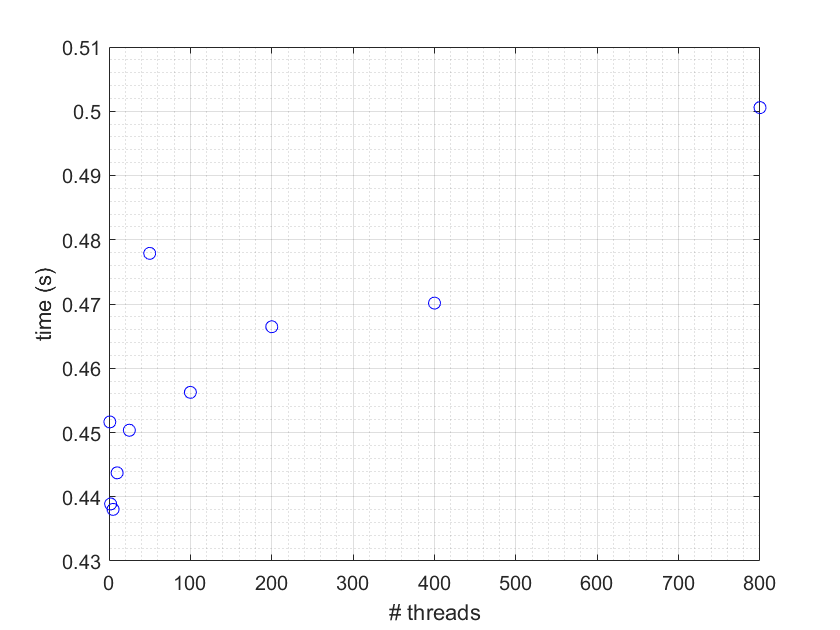
\includegraphics[scale=0.5]{./num_task_point}
  \caption{Execution time plot when varying the number of tasks (number of threads = 8).}
  \label{fig:num_task_point}
\end{figure}

Figure \ref{fig:num_task_point} shows the execution time of the program with a constant number of threads (8). The bigger the granularity (less number of tasks), the lower the execution time (and the lower speedup). The main reason is that we have to create less tasks. Thus, the overhead of creation and termination of tasks is smaller. The best option for this strategy is using small values for the number of tasks per row. In this situation, only 1 or 2 threads will execute the full row, while the other ones can execute the following rows.

\section{Row decomposition in OpenMP}

In this section, we are going to analyse the performance of the Row decomposition strategy using the best implementation we got with the Point strategy. Afterwards, we will compare both results. All versions of the codes can be found in files \textit{mandel-omp-task-row-taskloop-\{granularity\}-nogroup}.

The best implementation in the previous section was using the taskloop clause. Thus, the new code is the following:

\begin{figure}[H]
\begin{lstlisting}
#pragma omp parallel
#pragma omp single
#pragma omp taskloop firstprivate(row) num_tasks(800) nogroup
for (int row = 0; row < height; ++row) {
    for (int col = 0; col < width; ++col) {
        ...
	}
}
\end{lstlisting}
\caption{Fragment of the \textit{mandel-omp-task-row-taskloop-800-nogroup.c} code showing the OpenMP clauses to implement the task strategy with the taskloop variant.}
\label{code:task_implementation_row_taskloop_800}
\end{figure}

The following plots are the scalability plots using the same implementation but varying the number of tasks per row. They are only a part of all. The rest of the plots can be found in section \ref{sec:row_taskloop_scalability_plots}.


\begin{figure}[H]
\centering
\begin{minipage}[t]{0.4\linewidth}
  \centering
  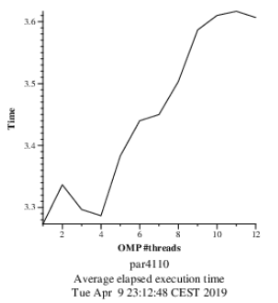
\includegraphics[scale=1.5]{./mandel-omp-10000-strong-omp-3-1-time}
  \caption{Execution time plot varying the number of threads (Num. tasks = 1).}
  \label{fig:mandel-omp-10000-strong-omp-3-1-time}
\end{minipage}%
\hspace{0.5cm}
\begin{minipage}[t]{0.4\linewidth}
  \centering
  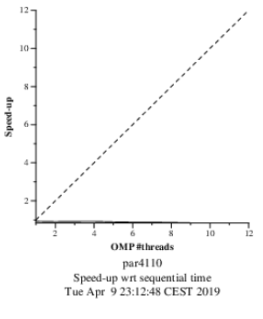
\includegraphics[scale=1.5]{./mandel-omp-10000-strong-omp-3-1-speedup}
  \caption{Speedup plot varying the number of threads (Num. tasks = 1).}
  \label{fig:mandel-omp-10000-strong-omp-3-1-speedup}
\end{minipage}
\end{figure}

\begin{figure}[H]
\centering
\begin{minipage}[b]{0.4\linewidth}
  \centering
  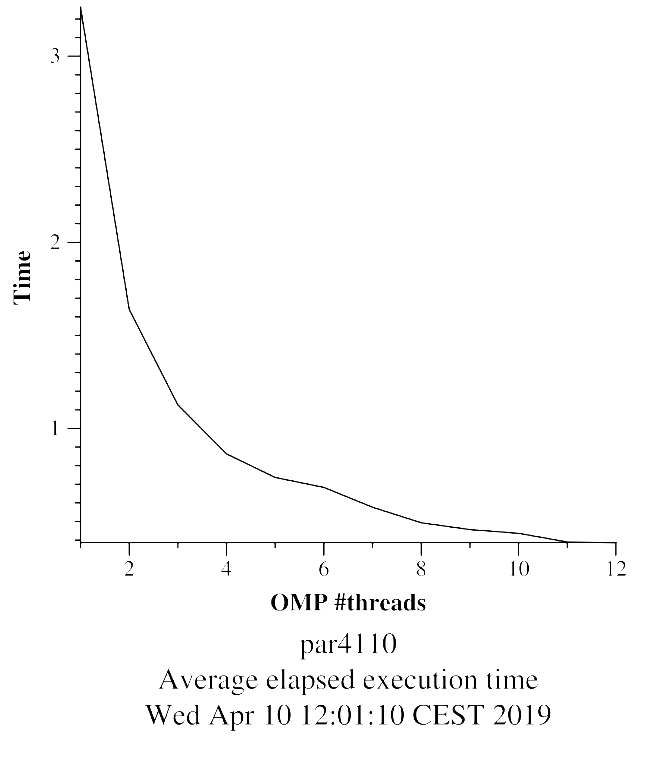
\includegraphics[scale=0.5]{./mandel-omp-10000-strong-omp-3-50-time}
  \caption{Execution time plot varying the number of threads (Num. tasks = 50).}
  \label{fig:mandel-omp-10000-strong-omp-3-50-time}
\end{minipage}%
\hspace{0.5cm}
\begin{minipage}[b]{0.4\linewidth}
  \centering
  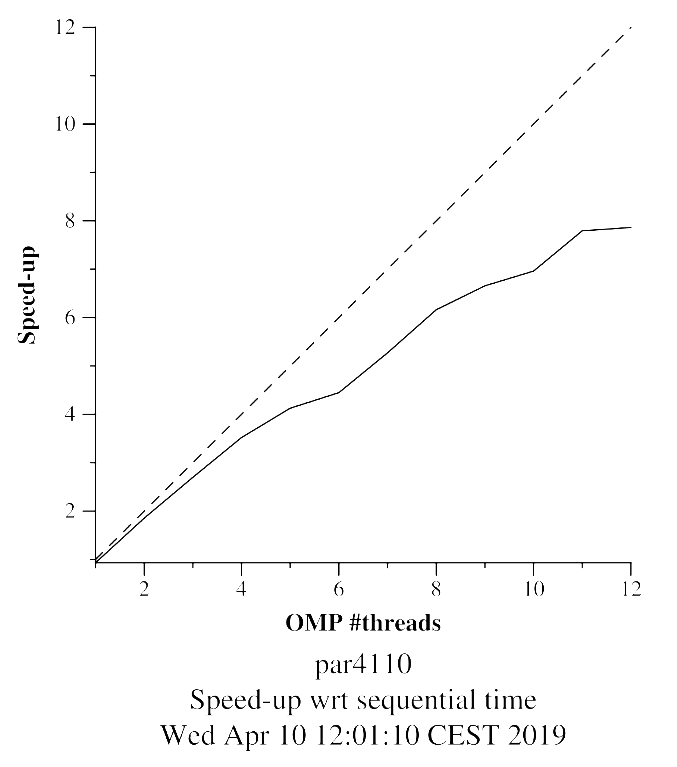
\includegraphics[scale=0.5]{./mandel-omp-10000-strong-omp-3-50-speedup}
  \caption{Speedup plot varying the number of threads (Num. tasks = 50).}
  \label{fig:mandel-omp-10000-strong-omp-3-50-speedup}
\end{minipage}
\end{figure}

\begin{figure}[H]
\centering
\begin{minipage}[b]{0.4\linewidth}
  \centering
  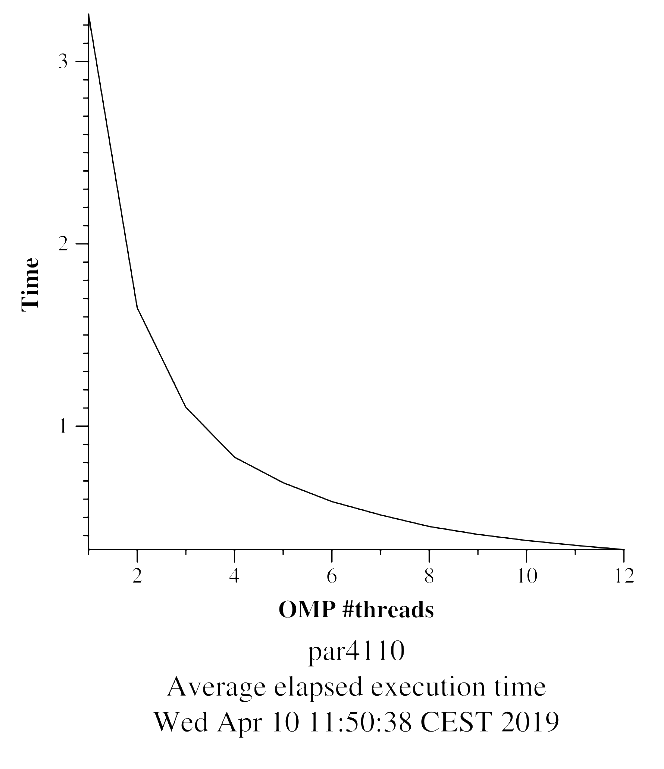
\includegraphics[scale=0.5]{./mandel-omp-10000-strong-omp-3-800-time}
  \caption{Execution time plot varying the number of threads (Num. tasks = 800).}
  \label{fig:mandel-omp-10000-strong-omp-3-800-time}
\end{minipage}%
\hspace{0.5cm}
\begin{minipage}[b]{0.4\linewidth}
  \centering
  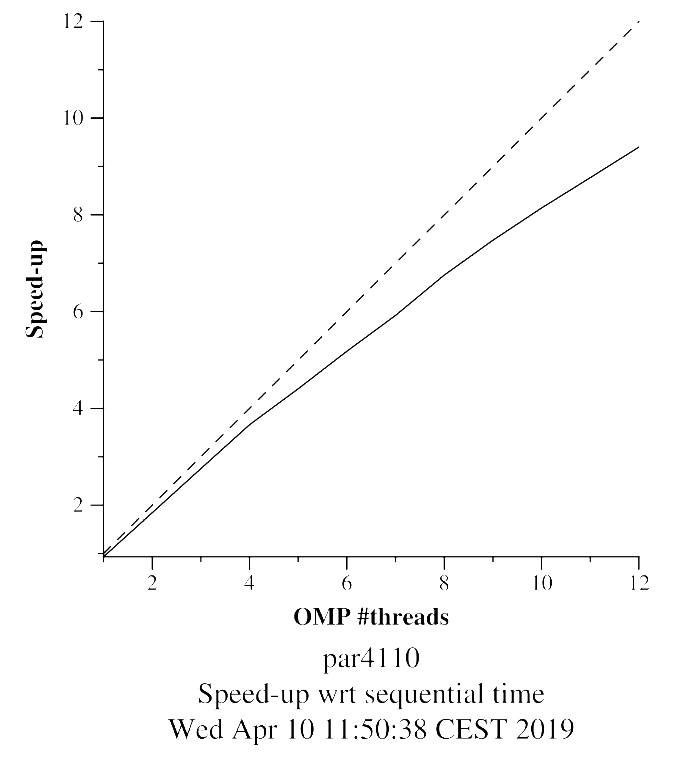
\includegraphics[scale=0.5]{./mandel-omp-10000-strong-omp-3-800-speedup}
  \caption{Speedup plot varying the number of threads (Num. tasks = 800).}
  \label{fig:mandel-omp-10000-strong-omp-3-800-speedup}
\end{minipage}
\end{figure}

We can see that now the tendency is the other way round with respect to the previous section. The bigger the number of tasks, the better the execution time. Now, the important thing is not the overhead but the distribution of the tasks into the different threads. Thus, a big number of tasks will balance better the work of the threads.

Now, in figure \ref{fig:num_task_row} we can see that the opposite happens. The bigger the granularity, the bigger the execution time. Thus, in the row strategy, the best option is to create as much tasks as possible. The main reason is that in this strategy, what we are modifying is the number of rows each thread executes. Hence, the bigger the number of tasks, the lower granularity (less intructions). This means that every thread will do less work per thread and will end faster, will take another task and so on.

\begin{figure}[H]
  \centering
  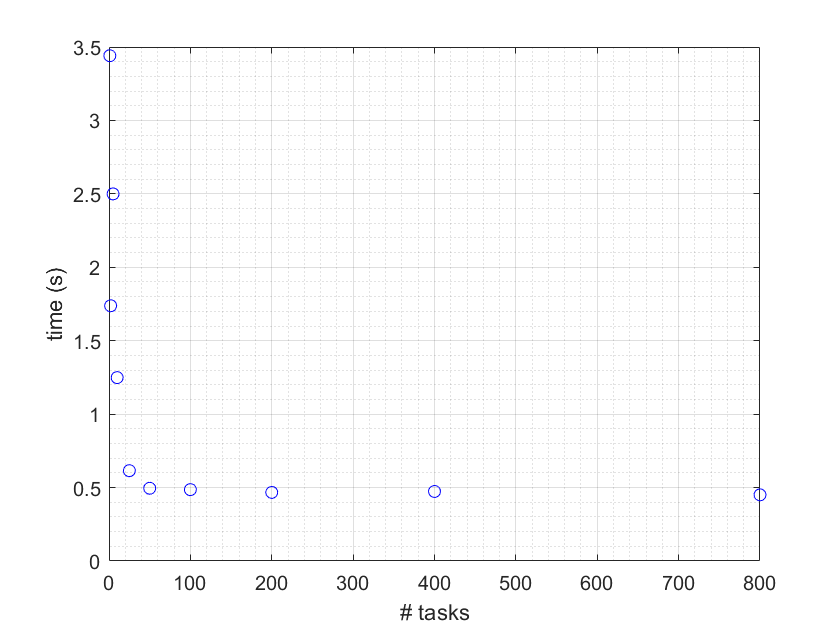
\includegraphics[scale=0.5]{./num_task_row}
  \caption{Execution time plot when varying the number of tasks (number of threads = 8).}
  \label{fig:num_task_row}
\end{figure}

%For the Row strategy implemented in OpenMP, describe the parallelization strategy that you have
%decided to implement. Reason about the performance that is obtained comparing with the results
%obtained for the best Point implementation, including the execution time and speed–up plots obtained
%in the strong scalability analysis (with -i 10000) and Paraver captures that help you to better explain
%the results that have been obtained.

\subsection{OpenMP For Implementation}

In this section, we are going to implement the for-based parallelization. With this new strategy, instead of tasking to distribute the work among the threads, we distribute loop iterations within the team of threads that encounters this work-sharing construct. The different codes can be found in the \textit{for} directory inside \textit{codes} directory.

\begin{figure}[H]
\begin{lstlisting}
#pragma omp parallel for schedule(static) private(col)
for (int row = 0; row < height; ++row) {
    for (int col = 0; col < width; ++col) {
    	...
    }
}
\end{lstlisting}
\caption{Fragment of the code \textit{mandel-omp-for-static.c}.}
\end{figure}

The following plots show the execution time and speedup for all possible schedules we know. We though that a value of 10 iterations per chunk would very accurate for a good solution. With a big number of iterations per chunk, as we are in the row strategy, one thread would have done a lot of work. Thus, the results would have been very bad.

\begin{figure}[H]
\centering
\begin{minipage}[b]{0.4\linewidth}
  \centering
  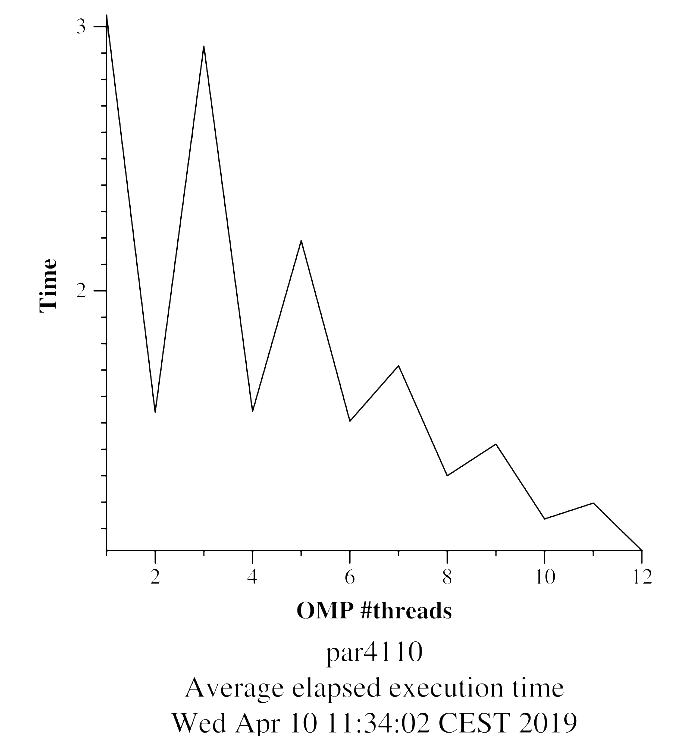
\includegraphics[scale=0.5]{./mandel-omp-10000-strong-omp-for-static-time}
  \caption{Execution time plot varying the number of threads (schedule(static)).}
  \label{fig:mandel-omp-10000-strong-omp-for-static-time}
\end{minipage}%
\hspace{0.5cm}
\begin{minipage}[b]{0.4\linewidth}
  \centering
  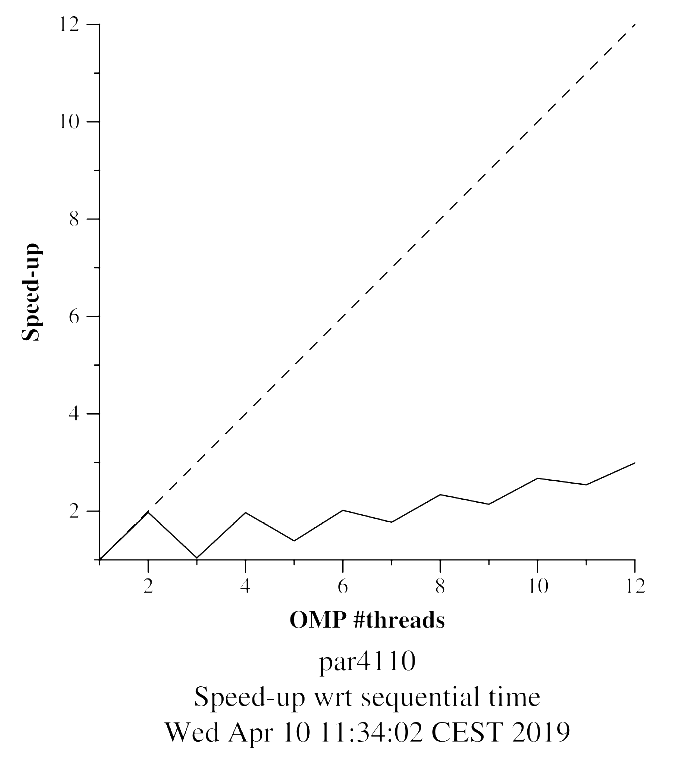
\includegraphics[scale=0.5]{./mandel-omp-10000-strong-omp-for-static-speedup}
  \caption{Speedup plot varying the number of threads (schedule(static)).}
  \label{fig:mandel-omp-10000-strong-omp-for-static-speedup}
\end{minipage}
\end{figure}

\begin{figure}[H]
\centering
\begin{minipage}[b]{0.4\linewidth}
  \centering
  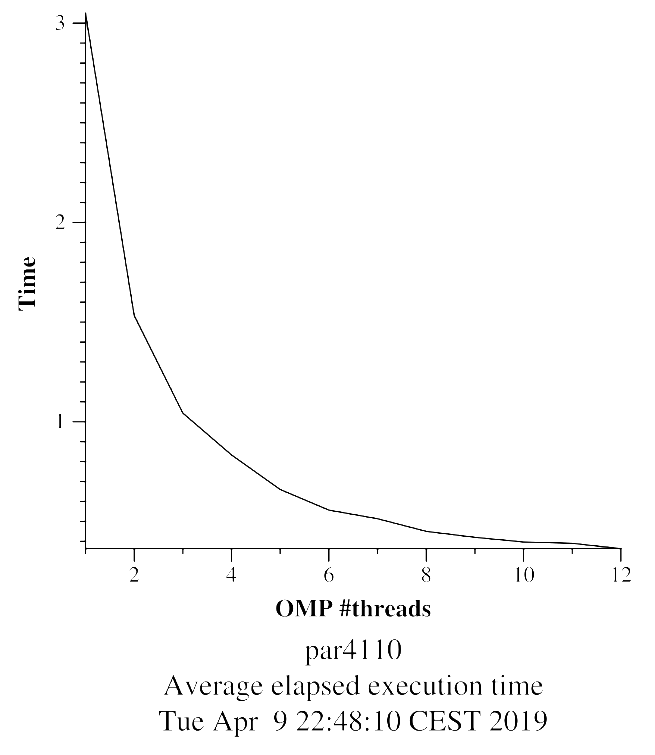
\includegraphics[scale=0.5]{./mandel-omp-10000-strong-omp-for-static-800-time}
  \caption{Execution time plot varying the number of threads (schedule(static, 10)).}
  \label{fig:mandel-omp-10000-strong-omp-for-static-800-time}
\end{minipage}%
\hspace{0.5cm}
\begin{minipage}[b]{0.4\linewidth}
  \centering
  \includegraphics[scale=0.5]{./mandel-omp-10000-strong-omp-for-static-800-speedup}
  \caption{Speedup plot varying the number of threads (schedule(static, 10)).}
  \label{fig:mandel-omp-10000-strong-omp-for-static-800-speedup}
\end{minipage}
\end{figure}

\begin{figure}[H]
\centering
\begin{minipage}[b]{0.4\linewidth}
  \centering
  \includegraphics[scale=0.5]{./mandel-omp-10000-strong-omp-for-dynamic-800-time}
  \caption{Execution time plot varying the number of threads (schedule(dynamic, 10)).}
  \label{fig:mandel-omp-10000-strong-omp-for-dynamic-800-time}
\end{minipage}%
\hspace{0.5cm}
\begin{minipage}[b]{0.4\linewidth}
  \centering
  \includegraphics[scale=0.5]{./mandel-omp-10000-strong-omp-for-dynamic-800-speedup}
  \caption{Speedup plot varying the number of threads (schedule(dynamic, 10)).}
  \label{fig:mandel-omp-10000-strong-omp-for-dynamic-800-speedup}
\end{minipage}
\end{figure}

\begin{figure}[H]
\centering
\begin{minipage}[b]{0.4\linewidth}
  \centering
  \includegraphics[scale=0.5]{./mandel-omp-10000-strong-omp-for-guided-800-time}
  \caption{Execution time plot varying the number of threads (schedule(guided, 10)).}
  \label{fig:mandel-omp-10000-strong-omp-for-guided-800-time}
\end{minipage}%
\hspace{0.5cm}
\begin{minipage}[b]{0.4\linewidth}
  \centering
  \includegraphics[scale=0.5]{./mandel-omp-10000-strong-omp-for-guided-800-speedup}
  \caption{Speedup plot varying the number of threads (schedule(guided, 10)).}
  \label{fig:mandel-omp-10000-strong-omp-for-guided-800-speedup}
\end{minipage}
\end{figure}

In figure \ref{fig:mandel-omp-for-schedule}, we can observe the different time executions when using only 8 threads. It is obvious that only static would be the one with a greater time execution because threads that have the tasks in the middle of the picture  have to do more iterations per pixel, as it is where most of the white pixels are located. However, if we use 10 iterations per chunk with the static schedule, the time is reduced a lot because now, all threads will execute tasks that have white pixels, so they will end faster.

On the other hand, the dynamic strategy is the best option because whenever one thread ends, OpenMP will give him another task of the same chunck size without losing time.

Finally, the guided strategy has not given the expected results. It is slower than schedule(static, 10). The reason is that with this strategy, we give a big number of iteration to each thread, until we arrive to the chunk size limit. Thus, some threads will have to execute tasks with a big number of white pixels.

\begin{figure}[H]
  \centering
  \includegraphics[scale=0.5]{./mandel-omp-for-schedule}
  \caption{Execution time plot for the different schedule methods.}
  \label{fig:mandel-omp-for-schedule}
\end{figure}

\newpage

\section{Conclusion}

In these 3 laboratory sessions we have seen different strategies and tasking methods on 2 nested loops.

We have found that the innermost loop iterations have different execution times because some points belong to the Mandelbrot set and others do not. Thus, some of them have to reach the maximum number of steps. 

This has led us to find that the best results in the Point strategy are obtained when tasks get a few number of iterations of the innermost loop.

On the other hand, the excessive creation of tasks leds us to an increment of the execution times due to that each task has a creation, synchronization and termination times.

Using different methods of creation of explicit tasks we have observed that the best method is using the taskloop clause because it leds us to control in an easier way the granularity of each task.

Moreover, we have seen that the best granularity for one strategy (for example, Point) is at the same time the worst granularity for the other strategy, and vice versa. The reason is because one strategy needs to create a lot of tasks to improve its parallelism (Row strategy) whereas the other one has to limit its creation of tasks due to the overhead (Point strategy).

Finally, we have seen that using implicit creation task in the Row strategy, the best option to use is the schedule(dynamic, 10) because it is the one that distributes better all the work.


\newpage

\section{Annex}

\subsection{Scalability plots of point strategy using taskloop implementation}
\label{sec:point_taskloop_scalability_plots}
\begin{figure}[H]
\centering
\begin{minipage}[b]{0.4\linewidth}
  \centering
  \includegraphics[scale=0.5]{./mandel-omp-10000-strong-omp-24-1-time}
  \caption{Execution time plot varying the number of threads (Num. tasks = 1).}
  \label{fig:mandel-omp-10000-strong-omp-24-1-time}
\end{minipage}%
\hspace{0.5cm}
\begin{minipage}[b]{0.4\linewidth}
  \centering
  \includegraphics[scale=0.5]{./mandel-omp-10000-strong-omp-24-1-speedup}
  \caption{Speedup plot varying the number of threads (Num. tasks = 1).}
  \label{fig:mandel-omp-10000-strong-omp-24-1-speedup}
\end{minipage}
\end{figure}

\begin{figure}[H]
\centering
\begin{minipage}[b]{0.4\linewidth}
  \centering
  \includegraphics[scale=0.5]{./mandel-omp-10000-strong-omp-24-2-time}
  \caption{Execution time plot varying the number of threads (Num. tasks = 2).}
  \label{fig:mandel-omp-10000-strong-omp-24-2-time}
\end{minipage}%
\hspace{0.5cm}
\begin{minipage}[b]{0.4\linewidth}
  \centering
  \includegraphics[scale=0.5]{./mandel-omp-10000-strong-omp-24-2-speedup}
  \caption{Speedup plot varying the number of threads (Num. tasks = 2).}
  \label{fig:mandel-omp-10000-strong-omp-24-2-speedup}
\end{minipage}
\end{figure}

\begin{figure}[H]
\centering
\begin{minipage}[b]{0.4\linewidth}
  \centering
  \includegraphics[scale=0.5]{./mandel-omp-10000-strong-omp-24-5-time}
  \caption{Execution time plot varying the number of threads (Num. tasks = 5).}
  \label{fig:mandel-omp-10000-strong-omp-24-5-time}
\end{minipage}%
\hspace{0.5cm}
\begin{minipage}[b]{0.4\linewidth}
  \centering
  \includegraphics[scale=0.5]{./mandel-omp-10000-strong-omp-24-5-speedup}
  \caption{Speedup plot varying the number of threads (Num. tasks = 5).}
  \label{fig:mandel-omp-10000-strong-omp-24-5-speedup}
\end{minipage}
\end{figure}

\begin{figure}[H]
\centering
\begin{minipage}[b]{0.4\linewidth}
  \centering
  \includegraphics[scale=0.5]{./mandel-omp-10000-strong-omp-24-10-time}
  \caption{Execution time plot varying the number of threads (Num. tasks = 10).}
  \label{fig:mandel-omp-10000-strong-omp-24-10-time}
\end{minipage}%
\hspace{0.5cm}
\begin{minipage}[b]{0.4\linewidth}
  \centering
  \includegraphics[scale=0.5]{./mandel-omp-10000-strong-omp-24-10-speedup}
  \caption{Speedup plot varying the number of threads (Num. tasks = 10).}
  \label{fig:mandel-omp-10000-strong-omp-24-10-speedup}
\end{minipage}
\end{figure}

\begin{figure}[H]
\centering
\begin{minipage}[b]{0.4\linewidth}
  \centering
  \includegraphics[scale=0.5]{./mandel-omp-10000-strong-omp-24-25-time}
  \caption{Execution time plot varying the number of threads (Num. tasks = 25).}
  \label{fig:mandel-omp-10000-strong-omp-24-25-time}
\end{minipage}%
\hspace{0.5cm}
\begin{minipage}[b]{0.4\linewidth}
  \centering
  \includegraphics[scale=0.5]{./mandel-omp-10000-strong-omp-24-25-speedup}
  \caption{Speedup plot varying the number of threads (Num. tasks = 25).}
  \label{fig:mandel-omp-10000-strong-omp-24-25-speedup}
\end{minipage}
\end{figure}

\begin{figure}[H]
\centering
\begin{minipage}[b]{0.4\linewidth}
  \centering
  \includegraphics[scale=0.5]{./mandel-omp-10000-strong-omp-24-50-time}
  \caption{Execution time plot varying the number of threads (Num. tasks = 50).}
  \label{fig:mandel-omp-10000-strong-omp-24-50-time}
\end{minipage}%
\hspace{0.5cm}
\begin{minipage}[b]{0.4\linewidth}
  \centering
  \includegraphics[scale=0.5]{./mandel-omp-10000-strong-omp-24-50-speedup}
  \caption{Speedup plot varying the number of threads (Num. tasks = 50).}
  \label{fig:mandel-omp-10000-strong-omp-24-50-speedup}
\end{minipage}
\end{figure}

\begin{figure}[H]
\centering
\begin{minipage}[b]{0.4\linewidth}
  \centering
  \includegraphics[scale=0.5]{./mandel-omp-10000-strong-omp-24-100-time}
  \caption{Execution time plot varying the number of threads (Num. tasks = 100).}
  \label{fig:mandel-omp-10000-strong-omp-24-100-time}
\end{minipage}%
\hspace{0.5cm}
\begin{minipage}[b]{0.4\linewidth}
  \centering
  \includegraphics[scale=0.5]{./mandel-omp-10000-strong-omp-24-100-speedup}
  \caption{Speedup plot varying the number of threads (Num. tasks = 100).}
  \label{fig:mandel-omp-10000-strong-omp-24-100-speedup}
\end{minipage}
\end{figure}

\begin{figure}[H]
\centering
\begin{minipage}[b]{0.4\linewidth}
  \centering
  \includegraphics[scale=0.5]{./mandel-omp-10000-strong-omp-24-200-time}
  \caption{Execution time plot varying the number of threads (Num. tasks = 200).}
  \label{fig:mandel-omp-10000-strong-omp-24-200-time}
\end{minipage}%
\hspace{0.5cm}
\begin{minipage}[b]{0.4\linewidth}
  \centering
  \includegraphics[scale=0.5]{./mandel-omp-10000-strong-omp-24-200-speedup}
  \caption{Speedup plot varying the number of threads (Num. tasks = 200).}
  \label{fig:mandel-omp-10000-strong-omp-24-200-speedup}
\end{minipage}
\end{figure}

\begin{figure}[H]
\centering
\begin{minipage}[b]{0.4\linewidth}
  \centering
  \includegraphics[scale=0.5]{./mandel-omp-10000-strong-omp-24-400-time}
  \caption{Execution time plot varying the number of threads (Num. tasks = 400).}
  \label{fig:mandel-omp-10000-strong-omp-24-400-time}
\end{minipage}%
\hspace{0.5cm}
\begin{minipage}[b]{0.4\linewidth}
  \centering
  \includegraphics[scale=0.5]{./mandel-omp-10000-strong-omp-24-400-speedup}
  \caption{Speedup plot varying the number of threads (Num. tasks = 400).}
  \label{fig:mandel-omp-10000-strong-omp-24-400-speedup}
\end{minipage}
\end{figure}

\begin{figure}[H]
\centering
\begin{minipage}[b]{0.4\linewidth}
  \centering
  \includegraphics[scale=0.5]{./mandel-omp-10000-strong-omp-24-800-time}
  \caption{Execution time plot varying the number of threads (Num. tasks = 800).}
  \label{fig:mandel-omp-10000-strong-omp-24-800-time}
\end{minipage}%
\hspace{0.5cm}
\begin{minipage}[b]{0.4\linewidth}
  \centering
  \includegraphics[scale=0.5]{./mandel-omp-10000-strong-omp-24-800-speedup}
  \caption{Speedup plot varying the number of threads (Num. tasks = 800).}
  \label{fig:mandel-omp-10000-strong-omp-24-800-speedup}
\end{minipage}
\end{figure}






\subsection{Scalability plots of row strategy using taskloop implementation}
\label{sec:row_taskloop_scalability_plots}

\begin{figure}[H]
\centering
\begin{minipage}[t]{0.4\linewidth}
  \centering
  \includegraphics[scale=1.5]{./mandel-omp-10000-strong-omp-3-1-time}
  \caption{Execution time plot varying the number of threads (Num. tasks = 1).}
  \label{fig:mandel-omp-10000-strong-omp-3-1-time}
\end{minipage}%
\hspace{0.5cm}
\begin{minipage}[t]{0.4\linewidth}
  \centering
  \includegraphics[scale=1.5]{./mandel-omp-10000-strong-omp-3-1-speedup}
  \caption{Speedup plot varying the number of threads (Num. tasks = 1).}
  \label{fig:mandel-omp-10000-strong-omp-3-1-speedup}
\end{minipage}
\end{figure}

\begin{figure}[H]
\centering
\begin{minipage}[b]{0.4\linewidth}
  \centering
  \includegraphics[scale=0.5]{./mandel-omp-10000-strong-omp-3-2-time}
  \caption{Execution time plot varying the number of threads (Num. tasks = 2).}
  \label{fig:mandel-omp-10000-strong-omp-3-2-time}
\end{minipage}%
\hspace{0.5cm}
\begin{minipage}[b]{0.4\linewidth}
  \centering
  \includegraphics[scale=0.5]{./mandel-omp-10000-strong-omp-3-2-speedup}
  \caption{Speedup plot varying the number of threads (Num. tasks = 2).}
  \label{fig:mandel-omp-10000-strong-omp-3-2-speedup}
\end{minipage}
\end{figure}

\begin{figure}[H]
\centering
\begin{minipage}[b]{0.4\linewidth}
  \centering
  \includegraphics[scale=0.5]{./mandel-omp-10000-strong-omp-3-5-time}
  \caption{Execution time plot varying the number of threads (Num. tasks = 5).}
  \label{fig:mandel-omp-10000-strong-omp-3-5-time}
\end{minipage}%
\hspace{0.5cm}
\begin{minipage}[b]{0.4\linewidth}
  \centering
  \includegraphics[scale=0.5]{./mandel-omp-10000-strong-omp-3-5-speedup}
  \caption{Speedup plot varying the number of threads (Num. tasks = 5).}
  \label{fig:mandel-omp-10000-strong-omp-3-5-speedup}
\end{minipage}
\end{figure}

\begin{figure}[H]
\centering
\begin{minipage}[b]{0.4\linewidth}
  \centering
  \includegraphics[scale=0.5]{./mandel-omp-10000-strong-omp-3-10-time}
  \caption{Execution time plot varying the number of threads (Num. tasks = 10).}
  \label{fig:mandel-omp-10000-strong-omp-3-10-time}
\end{minipage}%
\hspace{0.5cm}
\begin{minipage}[b]{0.4\linewidth}
  \centering
  \includegraphics[scale=0.5]{./mandel-omp-10000-strong-omp-3-10-speedup}
  \caption{Speedup plot varying the number of threads (Num. tasks = 10).}
  \label{fig:mandel-omp-10000-strong-omp-3-10-speedup}
\end{minipage}
\end{figure}

\begin{figure}[H]
\centering
\begin{minipage}[b]{0.4\linewidth}
  \centering
  \includegraphics[scale=0.5]{./mandel-omp-10000-strong-omp-3-25-time}
  \caption{Execution time plot varying the number of threads (Num. tasks = 25).}
  \label{fig:mandel-omp-10000-strong-omp-3-25-time}
\end{minipage}%
\hspace{0.5cm}
\begin{minipage}[b]{0.4\linewidth}
  \centering
  \includegraphics[scale=0.5]{./mandel-omp-10000-strong-omp-3-25-speedup}
  \caption{Speedup plot varying the number of threads (Num. tasks = 25).}
  \label{fig:mandel-omp-10000-strong-omp-3-25-speedup}
\end{minipage}
\end{figure}

\begin{figure}[H]
\centering
\begin{minipage}[b]{0.4\linewidth}
  \centering
  \includegraphics[scale=0.5]{./mandel-omp-10000-strong-omp-3-50-time}
  \caption{Execution time plot varying the number of threads (Num. tasks = 50).}
  \label{fig:mandel-omp-10000-strong-omp-3-50-time}
\end{minipage}%
\hspace{0.5cm}
\begin{minipage}[b]{0.4\linewidth}
  \centering
  \includegraphics[scale=0.5]{./mandel-omp-10000-strong-omp-3-50-speedup}
  \caption{Speedup plot varying the number of threads (Num. tasks = 50).}
  \label{fig:mandel-omp-10000-strong-omp-3-50-speedup}
\end{minipage}
\end{figure}

\begin{figure}[H]
\centering
\begin{minipage}[b]{0.4\linewidth}
  \centering
  \includegraphics[scale=0.5]{./mandel-omp-10000-strong-omp-3-100-time}
  \caption{Execution time plot varying the number of threads (Num. tasks = 100).}
  \label{fig:mandel-omp-10000-strong-omp-3-100-time}
\end{minipage}%
\hspace{0.5cm}
\begin{minipage}[b]{0.4\linewidth}
  \centering
  \includegraphics[scale=0.5]{./mandel-omp-10000-strong-omp-3-100-speedup}
  \caption{Speedup plot varying the number of threads (Num. tasks = 100).}
  \label{fig:mandel-omp-10000-strong-omp-3-100-speedup}
\end{minipage}
\end{figure}

\begin{figure}[H]
\centering
\begin{minipage}[b]{0.4\linewidth}
  \centering
  \includegraphics[scale=0.5]{./mandel-omp-10000-strong-omp-3-200-time}
  \caption{Execution time plot varying the number of threads (Num. tasks = 200).}
  \label{fig:mandel-omp-10000-strong-omp-3-200-time}
\end{minipage}%
\hspace{0.5cm}
\begin{minipage}[b]{0.4\linewidth}
  \centering
  \includegraphics[scale=0.5]{./mandel-omp-10000-strong-omp-3-200-speedup}
  \caption{Speedup plot varying the number of threads (Num. tasks = 200).}
  \label{fig:mandel-omp-10000-strong-omp-3-200-speedup}
\end{minipage}
\end{figure}

\begin{figure}[H]
\centering
\begin{minipage}[b]{0.4\linewidth}
  \centering
  \includegraphics[scale=0.5]{./mandel-omp-10000-strong-omp-3-400-time}
  \caption{Execution time plot varying the number of threads (Num. tasks = 400).}
  \label{fig:mandel-omp-10000-strong-omp-3-400-time}
\end{minipage}%
\hspace{0.5cm}
\begin{minipage}[b]{0.4\linewidth}
  \centering
  \includegraphics[scale=0.5]{./mandel-omp-10000-strong-omp-3-400-speedup}
  \caption{Speedup plot varying the number of threads (Num. tasks = 400).}
  \label{fig:mandel-omp-10000-strong-omp-3-400-speedup}
\end{minipage}
\end{figure}

\begin{figure}[H]
\centering
\begin{minipage}[b]{0.4\linewidth}
  \centering
  \includegraphics[scale=0.5]{./mandel-omp-10000-strong-omp-3-800-time}
  \caption{Execution time plot varying the number of threads (Num. tasks = 800).}
  \label{fig:mandel-omp-10000-strong-omp-3-800-time}
\end{minipage}%
\hspace{0.5cm}
\begin{minipage}[b]{0.4\linewidth}
  \centering
  \includegraphics[scale=0.5]{./mandel-omp-10000-strong-omp-3-800-speedup}
  \caption{Speedup plot varying the number of threads (Num. tasks = 800).}
  \label{fig:mandel-omp-10000-strong-omp-3-800-speedup}
\end{minipage}
\end{figure}

\end{document} 